% Run only with XeLaTeX!
%---------------------------------------------------------------------
%	FORMATING AND TYPESETTING
%---------------------------------------------------------------------

% Set document class
\documentclass[12pt,a4paper]{article}

% Option to change margin size
\usepackage[margin=2cm]{geometry}

% Font and encoding settings
\usepackage[T1]{fontenc}
%\usepackage[utf8]{inputenc} not necessary with xelatex?
\usepackage{yfonts} % germanic fonts (fraktur...)
%\defaultfontfeatures{Ligatures=TeX} %??

% Footnotes
\usepackage[stable]{footmisc}

% Indentation and spacing
\usepackage{indentfirst} % indentation
\usepackage{enumitem}[leftmargin=0pt] % spacing
\setlist{nosep}

% Formating of titles
\usepackage{titlesec}
\titleformat{\section}
{\normalfont\large\bfseries}{\thesection}{1em}{}
\titleformat{\subsection}
{\normalfont\normalsize\bfseries}{\thesubsection}{1em}{}
\titleformat{\subsubsection}
{\normalfont\small\bfseries}{\thesubsubsection}{1em}{}
\titleformat{\paragraph}[runin]
{\normalfont\small\bfseries}{\theparagraph}{1em}{}
\titleformat{\subparagraph}[runin]
{\normalfont\small\bfseries}{\thesubparagraph}{1em}{}
\usepackage[titletoc]{appendix}

% Math typesetting packages
\usepackage{amsmath, amssymb, amsthm, mathtools, commath}
\usepackage[warnings-off={mathtools-colon,mathtools-overbracket}]{unicode-math} % makes \mathbb{1} work and changes font of mathbb
\usepackage[mathscr]{euscript} % euler script font
\usepackage{tikz-cd} % tikz commutative diagrams

\AtBeginDocument{\renewcommand\setminus{\smallsetminus}} % \setminus doesn't work in unicode-math 

%---------------------------------------------------------------------


%---------------------------------------------------------------------
%	GRAPHICS
%---------------------------------------------------------------------

\usepackage{float}
\usepackage{caption}
\usepackage{graphicx}
\graphicspath{{images/}}

\usepackage{pdfpages} % for inserting pdf pages


%---------------------------------------------------------------------


%---------------------------------------------------------------------
%	BIBLIOGRAPHY
%---------------------------------------------------------------------

\usepackage[backend=biber,style=alphabetic]{biblatex}
\renewcommand*{\bibfont}{\small}
\addbibresource{thesis.bib}

%---------------------------------------------------------------------


%---------------------------------------------------------------------
%	HYPERLINKS
%---------------------------------------------------------------------

% Define the colors
\usepackage{xcolor}
\definecolor{brown}{HTML}{CD853F}
\definecolor{blue}{HTML}{4169E1}
\definecolor{green}{HTML}{2E8B57}

% Setup options for hyperlinks
\usepackage{hyperref}
\hypersetup{
colorlinks=true, linkcolor=black, breaklinks=true,
linktoc=all, bookmarksnumbered=true,
urlcolor=brown, linkcolor=blue, citecolor=green, % Link colors
}

% Referencing package
\usepackage{cleveref}
\crefname{section}{\S\!}{\S\S\!}
\Crefname{section}{\S\!}{\S\S\!}

%---------------------------------------------------------------------


%---------------------------------------------------------------------
%	THEOREM STYLES
%---------------------------------------------------------------------

% Define a dummy counter to keep count for all sub-environments
\newcounter{counter} \numberwithin{counter}{section}

% Define theorem styles here based on the definition style
\theoremstyle{definition}
\newtheorem{definition}[counter]{Definition}
\newtheorem{construction}[counter]{Construction}

% Define theorem styles here based on the plain style
\theoremstyle{plain} 
\newtheorem{theorem}[counter]{Theorem}
\newtheorem{corollary}[counter]{Corollary}
\newtheorem{lemma}[counter]{Lemma}
\newtheorem{proposition}[counter]{Proposition}
\newtheorem{conjecture}[counter]{Conjecture}

% Define theorem styles here based on the remark style
\theoremstyle{remark}
\newtheorem{example}[counter]{Example}
\newtheorem{remark}[counter]{Remark}

%---------------------------------------------------------------------


%---------------------------------------------------------------------
%	NEW COMMANDS
%---------------------------------------------------------------------

% general category
\newcommand{\catC}{\mathscr{C}}

% categories of factorization algebras
\newcommand{\falg}{\mathscr{F} \mathsf{Alg}}
\newcommand{\lcfa}{\mathscr{F} \mathsf{Alg}^{\mathsf{lc}}}

% category of manifolds
\newcommand{\mfld}[1][s]{%
    \ifx r#1\mathsf{Mfld}\else
    \ifx s#1\mathscr{M} \mathsf{fld}\else
    \mathrm{Illegal~option}%
    \fi\fi
}

% category of opens
\newcommand{\opens}[1][s]{%
    \ifx r#1\mathsf{Opns}\else
    \ifx s#1\mathscr{O} \mathsf{pns}\else
    \mathrm{Illegal~option}%
    \fi\fi
}

% category of Weiss cosheaves
\newcommand{\csheaves}{\mathsf{c} \mathscr{S} \mathsf{hv}^{\mathsf{W}}}

% category of disks
\newcommand{\disk}{\mathscr{D} \mathsf{isk}}

% category of infinity categories
\newcommand{\cat}{\mathscr{C} \mathsf{at}_{\infty}}

% template for category of algebras
\newcommand{\alg}[1]{\mathscr{A} \mathsf{lg}_{#1}}

% template for category of locally constant algebras
\newcommand{\lcalg}[1]{\mathscr{A} \mathsf{lg}^{\mathsf{lc}}_{#1}}

% half-open interval
\newcommand{\hoint}{\mathbb{R}_{\geq 0}}

% Cech complex
\newcommand{\cech}{\check{\mathsf{C}}}

% Automorphisms of category
\newcommand{\aut}{\mathsf{Aut}}

% Category of basics
\newcommand{\bsc}{\mathscr{B} \mathsf{sc}}
\newcommand{\bstr}{\mathscr{B}}


% Category of singular spaces
\newcommand{\snglr}{\mathscr{S} \mathsf{nglr}}


%---------------------------------------------------------------------

\setcounter{section}{-1}

\begin{document}

% Set title, author and date
\title{\texorpdfstring{\vspace*{5cm}}{}\sc Factorization Algebras and Factorization Homology on Stratified Spaces}
\author{Aleksandar Ivanov}
\date{06.09.2023}
\maketitle

\vspace{\fill}
\noindent
{\large \textbf{External UZH Supervisor:} Prof. Dr. Alberto Cattaneo}\\
{\large \textbf{External UZH Supervisor:} \"Od\"ul Tetik}\\
{\large \textbf{Internal ETH Supervisor:} Prof. Dr. Gian Michele Graf}\\ \\ \\ \\ \\ \\


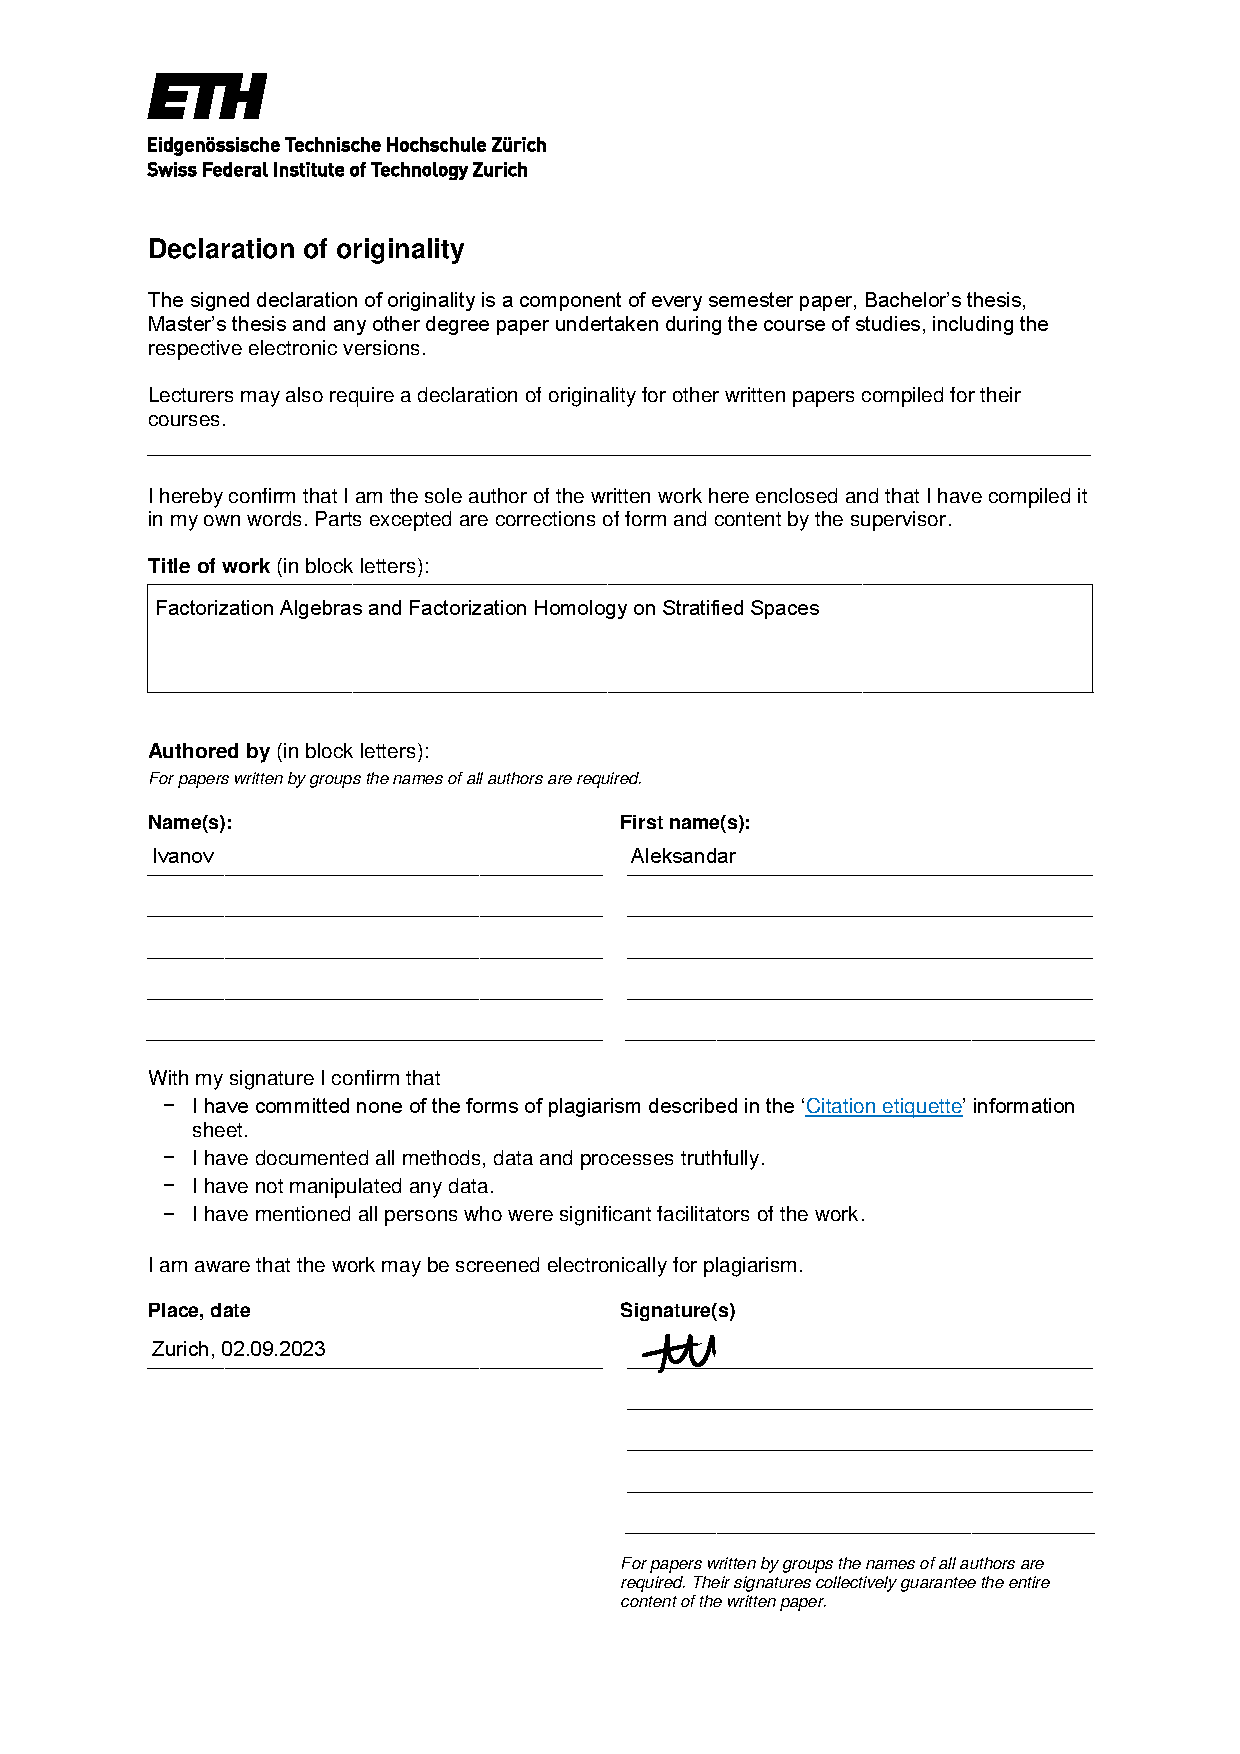
\includepdf[pages=-,pagecommand={},width=\textwidth]{declaration-originality-sgined.pdf}


\tableofcontents







\section{Introduction}

In this work we will explore the concepts of factorization algebras and factorization homology over stratified spaces. These two concepts, which at first sight will looks very different, will turn out to be closely related. We will try to keep the discussion on the level of stratified spaces, while pointing out which results have not yet been generalized. The outline of the text is as follows:

\textbf{Stratified spaces:} The first section, \cref{ch:strat_spaces}, deals with setting up the theory of stratified spaces. Beginning with the fundamentals which have existed since the work of Whitney \cite{whitney92}. The particular version of stratified spaces that we use will be due to Ayala, Francis and Tanaka \cite{aft_localstrut}. This is because they can define a notion of conical smoothness, that is the equivalent to smoothness of unstratified manifolds. We will not go into the full details that this incarnation of the theory has to offer, but instead we will only focus on the results that we will make use of later on. Beyond, conical smoothness, this will include tangential structure and its stratified generalization, together with the packaging of both of these data into the concept of an $\infty$-category of basic singularity types.

\textbf{Factorization Homology:} The second section, \cref{ch:fact_hom}, will present the theory of factorization homology. For this purpose we will need the concept of (structured) disk algebras, since this will be the algebraic input of the theory. Factorization homology will then return an invariant of a manifold. We will explore the key example of factorization homology over the closed, oriented, interval, and see how this gives rise to the algebraic concept of the two-sided bar construction. More generally, this underpins the theory because it codifies the property of $\otimes$-excision, and what it means to be a homology theory. Finally, we will also state a classification result about a certain type of disk algebras with stratified structure.

\textbf{Factorization Algebras:} The third section, \cref{ch:fact_alg}, introduces the concept of factorization algebras, with its various subtypes, like prefactorization algebras and locally constant factorization algebras. We will see that, of these, the locally constant ones are those that can see the possible stratified structure of the underlying space. After introducing the pushforward of factorization algebras, we will spend some time on finding ways to construct factorization algebras from fewer data than the original definition requires. This will introduce factorization homology back into the picture, and we will see the relation between the two. Finally, we will examine some examples of factorization algebras whose construction is known.

\textbf{Collar-gluings and Disk Algebras:} The fourth section, \cref{ch:gluing_disk_alg}, presents a novel result about the behavior of certain types of disk algebras under the operation of collar-gluing. It essentially shows that once can reproduce a disk algebra on a stratified manifold if we know it on some particular pieces of it together with the data of how to glue them. In the smooth case the result directly extends to locally constant factorization algebras, in which case it gives a way to calculate the $\infty$-category of factorization algebras on the spheres $S^n$ in particular.

\textbf{Classifying $\lcfa$s on Defect Manifolds:} The fifth section, \cref{ch:classif_defect_mfld}, presents a roadmap towards a classification of locally constant factorization algebras on a particular family of stratified manifolds; the ones with a distinguished, properly, embedded submanifold (defect). While we cannot reach a full classification, we do make observations that simplify the problem.

\textbf{Applications to Physical Examples:} The final, sixth, section, \cref{ch:physics}, presents a small sliver of the relationship between factorization algebras and structures that arise in physics, based on the work \cite{cg2016}. In particular, it argues that the factorization algebras are the natural structure for the observables of a quantum theory.

\textbf{Acknowledgements:} I would like to thank my partner, Rebecca, for your patience and understanding. This work wouldn't have been possible without your support. I would like to thank my supervisors for their guidance during this thesis and beyond. The conversations with \"Od\"ul Tetik, in particular, formed the basis of my understanding of the topic. I am grateful for the time he put into teaching me and focusing my attention.

\subsection{Conventions on \texorpdfstring{$\infty$}{infinity}-categories}

The $\infty$-categories in this work will use the quasi-category model of $\infty$-category theory introduced by Joyal in \cite{joyal}, which is based on the simplicial sets introduced by \cite{bv73}. The work by Lurie in \cite{lurie_htt} and \cite{lurie_ha} greatly builds on this theory, and questions about fundamental objects or constructions that are in this text will always be answered in those references. This choice is because a great deal of the theory of factorization homology, as well as factorization algebras deal with $\infty$-categories of functors, which are most easily defined for quasi-categories.

It is also important to note that we will not be making a notational distinction between topological categories, Kan enriched categories and $\infty$-categories because of the functors
%
\begin{align}
    \{ \mathsf{Top}\mathrm{-categories}\} \xrightarrow{\mathsf{Sing}} \{ \mathsf{Kan}\mathrm{-categories}\} \xrightarrow{\mathsf{N}} \cat,
\end{align}
%
which are both equivalences in appropriate ways. In particular, we will not distinguish the nerve of an ordinary category from the ordinary category itself.










\section{Stratified Spaces}\label{ch:strat_spaces}

The spaces that this work will be set in will very often be stratified spaces. Thus, we first need to define what we mean by this concept. There are multiple definitions of stratified spaces in the literature, all of which have their advantages and disadvantages. For our purposes, we will follow the account of \cite{aft_localstrut}. The majority of the work on factorization homology has so far been elaborated using this particular set of definitions, and similarly the stratified spaces used in the literature on factorization algebras are usually subsumed too. Here we will only recap the results that will be of use to us. Further details are, of course, discussed in \cite{aft_localstrut}, where one can find a great explanation of the definitions that are needed, and detailed proofs of the theorems that can be proven.

\subsection{Fundamentals of Stratified Spaces}

\begin{definition}
    We will regard posets as topological spaces by declaring that a map $P \rightarrow P'$ is continuous if, any only if it is a map of posets. This means that we declare a subset $U \subset P$ to be open if for all $a \in U$, any $b \geq a$ is also in $U$. This gives a fully faithful functor
    %
    \begin{align}
        \mathsf{Poset} \xhookrightarrow{} \mathsf{Top}.
    \end{align} 
\end{definition}

\begin{definition}[\cite{lurie_ha}]
    Let $P$ be a poset. A \emph{$P$-stratified space} is a topological space $X$ together with a map $X \rightarrow P$, which we call the stratification of $X$. We will sometimes refer to $X$ as the underlying topological space of a stratified space. Furthermore, we denote the preimage of $p \in P$ as $X_p$ and call it the $p$th stratum of $X$.
\end{definition}

\begin{example}
    Any CW complex $X$ can be made into a stratified space $X \rightarrow \mathbb{N}$, which sends all points in $X_{\leq k} \setminus {X_{\leq k-1}}$ to $k$, where $X_{\leq k}$ is the $k$-skeleton of $X$.
\end{example}

\begin{example}
    Inspired by the previous example, any topological space $X$ with a filtration by closed subsets $\emptyset \subset X_{\leq 0} \subset \dots \subset X_{\leq n} = X$, is a stratified space, because the filtration induces a map $X \rightarrow \mathbb{N}$, which sends $X_{\leq i} \setminus X_{\leq i-1}$ to $i$.
\end{example}

\begin{remark}
    Given two stratified spaces $X \xrightarrow{s} P$ and $X' \xrightarrow{s'} P'$, we can form the product stratified space $X \times X' \xlongrightarrow{s \times s'} P \times P'$, where the partial order on the product poset is given by $(p,p') \leq (q, q') \iff (p \leq q) \land (p' \leq q')$.
\end{remark}

\begin{example}
    Consider the poset $[1] = \{0 < 1\}$, and the topological space $\hoint$. The standard stratification that we will give to this space is given by $\hoint \rightarrow [1]$, that sends $0 \mapsto 0$ and $0 \neq x \mapsto 1$. This space will play an important role for factorization algebras later on.
\end{example}

\begin{definition}
    Let $X \rightarrow P$ and $X' \rightarrow P'$ be two stratified spaces. A \emph{continuous stratified map} (or \emph{map of stratified spaces}) is a commutative diagram in $\mathsf{Top}$
    %
    \begin{center}
        \begin{tikzcd}
            X \arrow[r] \arrow[d] & X' \arrow[d] \\
            P \arrow[r] & P'.
        \end{tikzcd}
    \end{center}
\end{definition}

\begin{example}\label{ex:forget_strat}
    Every stratified space $(X \rightarrow P)$ has a continuous stratified map that forgets the stratification $(X \rightarrow P) \rightarrow (X \rightarrow *)$, giving data equivalent to an unstratified topological space. 
\end{example}

\begin{definition}
    A continuous stratified map $(f: X \rightarrow X', g: P \rightarrow P')$ is an \emph{open embedding} if $f: X \rightarrow X'$ is an open embedding of topological spaces.
\end{definition}

\begin{remark}
    The above definitions give us a natural notion of an open cover $\{ (U_i \rightarrow P_i) \xhookrightarrow{} (X \rightarrow P)\}_{i \in I}$ of a stratified space $(X \rightarrow P)$, namely, whenever both $\{ U_i \xhookrightarrow{} X\}_{i \in I}$ and $\{ P_i \xhookrightarrow{} P \}_{i \in I}$ are open covers.
\end{remark}

Next, we construct the cone of a stratified space. This plays a very important role in the theory of stratified manifolds, since the neighborhoods of these spaces will always look like a cone over some space with a possible further thickening by some $\mathbb{R}^k$. That is, the cones will be the model space for singularities.

\begin{definition}
    Let $X \rightarrow P$ be a stratified space. The cone $\mathsf{C}(X \rightarrow P)$ is the stratified space constructed as follows. At the level of topological spaces we define the pushout in $\mathsf{Top}$
    %
    \begin{align}
        \mathsf{C}(X) := * \coprod_{X \times \{0\}} X \times \hoint.
    \end{align}
    %
    At the level of posets we define the pushout in $\mathsf{Poset}$
    %
    \begin{align}
        \mathsf{C}(P) := * \coprod_{P \times \{ 0\}} P \times [1].
    \end{align}
    %
    The standard stratification of $\hoint$ together with the obvious map $* \rightarrow *$ induce a stratification $\mathsf{C}(X) \rightarrow \mathsf{C}(P)$ as a map between pushouts. 
\end{definition}

The equivalent of a topological manifold in the stratified setting is a \emph{$C^0$ stratified space}. We will not be fully precise in the definition of these, since this would stray us from our main goal. We will however cite theorems that show that the spaces we consider in this work are $C^0$ stratified spaces. The reason why the below cannot be the actual definition is because it would partially be a cyclic statement. We cite it because it provides good intuition for the structure of $C^0$ stratified spaces.

\begin{definition}
    A \emph{$C^0$ basic} is a $C^0$ stratified space of the form $\mathbb{R}^k \times \mathsf{C}(Z)$, where $k \geq 0$, $\mathbb{R}^k$ has the trivial stratification, and $Z$ is a compact $C^0$ stratified space.
\end{definition}

\begin{theorem}[{\cite[lem.2.2.2]{aft_localstrut}}]\label{thm:basics_give_basis}
    Let $X$ be a stratified, second countable, Hausdorff space, and consider the collection of open embeddings
    %
    \begin{align}
        \{ U \xhookrightarrow{} X\},
    \end{align}
    %
    where $U$ ranges over the $C^0$ basics. Then this collection forms a basis for the topology of $X$ if and only if $X$ is a $C^0$ stratified space.
\end{theorem}

\begin{theorem}[{\cite[cor.2.3.5]{aft_localstrut}}]
    Let $X \rightarrow P$ be a $C^0$ stratified space. For any $p \in P$, the stratified spaces $X_{\leq p}$, $X_{p}$ and $X_{\nless p}$, defined as the relevant preimages, are $C^0$ stratified spaces. Furthermore, $X_p$ is even a topological manifold.
\end{theorem}

\begin{remark}
    Because of the above theorem, $C^0$ stratified spaces $X \rightarrow P$ have a natural filtration by dimension since there is a map $P \rightarrow \mathbb{N}$, which sends $p \mapsto \mathsf{dim}(X_p)$. In our examples of interest we will always choose dimension as the stratification.
\end{remark}


The smooth version of the above concepts also exists and will be the one that is of main interest. As was the case for $C^0$ stratified spaces, we will not give the precise definition of a \emph{conically smooth stratified space} (or \emph{stratified manifold} for short), since the exact definition is involved. The idea, though, is the same as for smooth manifolds.

A stratified manifold is a $C^0$ stratified space $M$ equipped with an atlas
%
\begin{align}
    \{\mathbb{R}^{k_\alpha} \times \mathsf{C}(Z_\alpha) \hookrightarrow M\}_\alpha,
\end{align}
%
whose elements we call basics. This atlas has to be a basis for the topology of $X$, and the transitions maps, open embeddings among basics, have to be conically smooth. General maps of stratified manifolds will then be conically smooth if their representatives in basics are conically smooth.

The reason why the definition is involved is, because unlike in the smooth case the presence of the compact spaces $Z_\alpha$ means that we have to use induction to define conical smoothness.

In lieu of a definition we give the following illuminating example:
%
\begin{example}
    Smooth manifolds fall under the definition of stratified manifolds as those that only have one stratum. A smooth map $f$ between compact smooth manifolds gives rise to a conically smooth map $\mathsf{f}$ between the cones of these manifolds. If we also have a smooth map between Euclidean spaces $g$ then the map $h \times \mathsf{C}(f)$ is also conically smooth. This already allows us to describe stratified manifolds with two strata.
\end{example}

The next    classes of conically smooth maps will be present throughout this work.

\begin{definition}
    Let $f: M \rightarrow N$ be a conically smooth map.
    %
    \begin{enumerate}
        \item $f$ is an \emph{open embedding} if it is an open map that is conically diffeomorphic onto its image.
        \item $f$ is a \emph{refinement} if it's a homeomorphism of underlying topological spaces, and it's restriction to each stratum of $M$ is an embedding.
        \item Let $P_N$ be the stratifying poset of $N$. $f$ is a \emph{constructible bundle} if, for each $p \in P_N$, the restriction $f|_p: M|_{f^{-1} N_p} \rightarrow N_p$ is a fiber bundle of stratified spaces.
    \end{enumerate}
\end{definition}

\begin{remark}
    We will also on occasion use the concept of \emph{weakly constructible bundle}, which is a continuous stratified map $f: M \rightarrow N$ which is a constructible bundle out of a refinement of $M$, i.e. there is a diagram $M \xleftarrow{r} M' \xrightarrow{f'} N$, where there is an equality $f = f' \circ r$ of the underlying continuous maps. Constructible bundles are obviously also weakly constructible.
\end{remark}

For the next definition we notice that all standard simplices are stratified manifolds.

\begin{definition}
    $\snglr$ is the $\infty$-category whose objects are stratified manifolds and whose morphisms are open embeddings among them. To get the higher categorical structure we consider a simplicial enrichment over $\mathsf{Set}$-valued presheaves on the unenriched category, so that given two objects $M$ and $N$
    %
    \begin{align}
        \mathsf{Hom}_{\snglr} (M, N): [p] \mapsto \mathsf{S}_{/\Delta^p} (M \times \Delta^p, N \times \Delta^p),
    \end{align}
    %
    where $\Delta^p$ is the standard $p$-simplex and $\mathsf{S}_{/\Delta^p}$ denotes those stratified maps that commute with projecting to $\Delta^p$. It can be shown that this enrichment factors through a $\mathsf{Kan}$-enrichment, which gives the appropriate structure.
\end{definition}

\begin{remark}
    The above definition is not immediately parsable, but it can be shown that reducing to the case of smooth manifolds this definition gives equivalent data to the topological enrichment which to morphism spaces assigns the compact-open topology. 
\end{remark}

\begin{definition}
    The $\infty$-category of basic singularity types $\bsc \subset \snglr$ is the full $infty$-subcategory of those objects that are basics.
\end{definition}




\subsection{Stratified Manifolds with Tangential Structure}

In a lot of cases we will want to add to our stratified manifold the data of tangential structure. This, for example, will be the geometric input for factorization homology. Thus, we introduce the concept of tangential structure here, first starting with smooth manifolds and then continuing to the stratified case.

\begin{definition}
    Let $\mfld_n$ be the $\infty$-category defined as a topological category, whose objects are smooth, $n$-dimensional manifolds and whose morphisms are embeddings between them, where the morphism spaces have the compact-open topology. This category can be endowed with a symmetric monoidal structure given by disjoint union.
\end{definition}

Given a smooth, $n$-dimensional manifold $M$, its tangent bundle is a rank-$n$ vector bundle on the manifold, which also makes it a principal $\mathsf{GL}(n)$-bundle. Because of the classification of principal bundles, the tangent bundle of a manifold $M$ can be classified, up to homotopy, by a map called the \emph{tangent classifier}
%
\begin{align}
    M \xrightarrow{\ \ \tau_M \ \ } \mathsf{BO}(n) \xrightarrow[\simeq]{\mathrm{Gram-Schmidt}} \mathsf{BGL}(n),
\end{align}
%
where $\mathsf{BO}(n)$ is the classifying space of $\mathsf{O}(n)$. Giving the manifold a $G$-structure, where $G$ is a Lie group with a group homomorphism to $\mathsf{GL}(n)$, is then equivalent to a factorization, up to homotopy, of the tangent classifier through $\mathsf{B}G$, in other words it is a lift $\phi$ of the tangent classifier such that the following diagram is homotopy commutative
%
\begin{center}
    \begin{tikzcd}[column sep = large]
        & \mathsf{B}G \arrow[d] \\
        M \arrow[ru, dashed, "\phi"] \arrow[r, "\tau_M"] & \mathsf{BO}(n).
    \end{tikzcd}
\end{center}

It is, in fact, this picture that will generalize to give us tangential structure in the more general case. As a first step, \cite[cor.2.13]{af_fhtop} shows that the tangent classifier can be understood as a functor
%
\begin{align}
    \tau: \mfld_n \xrightarrow{\mathrm{Yoneda}} \mathsf{PShv}(\mfld_n) \xrightarrow{-|_{\mathbb{R}^n \subset \mfld_n}} \mathsf{PShv}(\mathbb{R}^n) \simeq \mathsf{Spaces}_{/\mathsf{BO}(n)},
\end{align}
%
and in fact a symmetric monoidal one, where the codomain's symmetric monoidal structure is given by coproduct. Namely, given a smooth manifold $M$, the functor returns the map of spaces $\tau_M:M \rightarrow \mathsf{BO}(n)$.

By fixing a space $B$ with a map $B \rightarrow \mathsf{BO}(n)$ (the role of which was previously played by $\mathsf{B}G$), we can define:
%
\begin{definition}
    The symmetric monoidal $\infty$-category $\mfld_n^B$ of $n$-manifolds with $B$-structure is the pullback of $\infty$-categories
    %
    \begin{center}
        \begin{tikzcd}
            \mfld_n^B \arrow[dr, phantom, "\ulcorner", very near start] \arrow[r] \arrow[d] & \mathsf{Spaces}_{/B} \arrow[d] \\
            \mfld_n \arrow[r, "\tau"] & \mathsf{Spaces}_{/\mathsf{BO}(n)},
        \end{tikzcd}
    \end{center}
    %
    where the right vertical arrow is induced by the map $B \rightarrow \mathsf{BO}(n)$.
\end{definition}

\begin{remark}
    Since the tangent classifier $\tau$ is symmetric monoidal, and since the right vertical map is canonically symmetric monoidal with the coproduct on both $\mathsf{Spaces}_{/B}$ and $\mathsf{Spaces}_{/\mathsf{BO}(n)}$, the newly defined $\infty$-category does indeed come with a canonical symmetric monoidal structure.
\end{remark}

\begin{example}
    Classical examples for tangential structure come from principal $G$-bundles as discussed before. Namely, given a Lie group $G$ together with a smooth homomorphism $G \rightarrow \mathsf{GL}(n) \simeq \mathsf{O}(n)$, we have an induced map of spaces $\mathsf{B}G \rightarrow \mathsf{BO}(n)$, which gives rise to the following examples:
    %
    \begin{enumerate}
        \item $(G \rightarrow \mathsf{O}(n)) = (\mathsf{O}(n) \xrightarrow{\mathrm{id}} \mathsf{O}(n))$ reproduces the case of no tangential structure,
        \item $(G \rightarrow \mathsf{O}(n)) = (\mathsf{SO}(n) \xhookrightarrow{} \mathsf{O}(n))$ is the case of oriented smooth manifolds,
        \item $(G \rightarrow \mathsf{O}(n)) = (\mathsf{Spin}(n) \rightarrow \mathsf{SO}(n) \xhookrightarrow{} \mathsf{O}(n))$ is the case of spin structure,
        \item $(G \rightarrow \mathsf{O}(n)) = (* \rightarrow \mathsf{O}(n))$ is the case of framed smooth manifolds.
    \end{enumerate}
\end{example}

Moving on to the stratified setting, we note that the stratified version of the full $\infty$-subcategory $\mathbb{R}^n \subset \mfld_n$ is the $\infty$-category of basic singularity types $\bsc$. We can thus generalize the tangent classifier to this setting as the functor
%
\begin{align}
    \tau: \snglr \xrightarrow{\mathrm{Yoneda}} \mathsf{PShv}(\snglr) \xrightarrow{-|_{\bsc \subset \snglr}} \mathsf{PShv}(\bsc).
\end{align}
%
In this case, as in the previous, given a stratified manifold $M$, $\tau(M)$ is the functor that for each basic $U \in \bsc$, assigns the space of stratified smooth open embeddings of $U$ into $M$.

\begin{remark}\label{rem:grothendieck_construction}
    We can say something more about this situation if we use the unstraightening construction \cite[sec.2.2]{lurie_htt} which provides an equivalence between $\mathsf{Spaces}$-valued presheaves on a general $\infty$-category $\catC$ and right fibrations \footnote{More details can be found in the cited references, but for completeness we include the definition of right fibration. A \emph{right fibration} (over $\catC$) is a functor $f:\mathscr{E} \rightarrow \catC$ such that the diagram
    %
    \begin{center}
        \begin{tikzcd}[ampersand replacement=\&]
            \Lambda^n_i \arrow[r] \arrow[d, hook] \& \mathscr{E} \arrow[d] \\
            \Delta^n \arrow[r] \arrow[ru, dashed] \& \catC        
        \end{tikzcd}
    \end{center}
    %
    can be filled for any $0 < i \leq n$.} over this $\infty$-category
    %
    \begin{align}
        \mathsf{PShv}(\catC) \simeq \mathsf{RFib}_{\catC}.
    \end{align}
    %
    More details on this equivalence in our context can be found in \cite[sec.4.2]{aft_localstrut}
    Appending this equivalence to the definition of the tangent classifier would say that the value of the tangent classifier on a stratified manifold $M$ is given by the right fibration
    %
    \begin{align}
        \tau_M: \mathsf{Entr}(M) := \bsc_{/M} \rightarrow \bsc,
    \end{align}
    %
    i.e. the forgetful functor from the slice $\infty$-category. The $\infty$-category $\mathsf{Entr}(M)$ defined here is called the enter-path $\infty$-category of the stratified manifold $M$\footnote{A different version of this $\infty$-cateogry is defined in \cite[app.A.6]{lurie_ha} called the exit-path $\infty$-category of the stratified space $M$. It is shown in the work \cite{afr_homhyp} that this exit-path $\infty$-category is equivalent to the opposite of the enter-path $\infty$-category as defined above.}. In fact the statements that we will make next will take on this perspective for the tangent classifier.
\end{remark}

Having generalized the tangent classifier to stratified manifolds we can now think about adding structure to them. The key realization is that the data which the map of spaces $B \rightarrow \mathsf{BO}(n)$ provided before was the data of a presheaf on $\mathsf{BO}(n)$, standing in as the $\infty$-category of basics with only one object $\mathbb{R}^n$. The analogous construction in the stratified case is to provide a presheaf on $\bsc$, which by \cref{rem:grothendieck_construction} is given by a right fibration over $\bsc$. 

\begin{definition}
    An $\infty$-category of basics is a right fibration $\bstr \rightarrow \bsc$
\end{definition}

\begin{definition}
    Given an $\infty$-category of basics $\bstr \rightarrow \bsc$, the $\infty$-category of $\bstr$-manifolds is the pullback
    %
    \begin{center}
        \begin{tikzcd}
            \mfld(\bstr) \arrow[dr, phantom, "\ulcorner", very near start] \arrow[r] \arrow[d] & (\mathsf{RFib}_{\bsc})_{/\bstr} \arrow[d] \\
            \snglr \arrow[r, "\tau"] & \mathsf{RFib}_{\bsc}.
        \end{tikzcd}
    \end{center}
\end{definition}

\begin{remark}
    Specifying to the objects of $\mfld(\bstr)$, we have that a $\bstr$-manifold is a stratified manifold $M$ together with a lift $\phi$
    %
    \begin{center}
        \begin{tikzcd}[column sep = large]
            & \bstr \arrow[d] \\
            \mathsf{Entr}(M) \arrow[ru, "\phi"] \arrow[r, "\tau_M"] & \bsc,
        \end{tikzcd}
    \end{center}
    %
    i.e. such that the triangle above is homotopy commutative in the $\infty$-category of $\infty$-categories $\cat$. This is how we can encode the stratification information while keeping the basic idea of a lift the same.
\end{remark}

\begin{remark}
    There is an obvious, fully faithful inclusion $\bstr \xhookrightarrow{} \mfld(\bstr)$, just as there was in the case without tangential structure.
\end{remark}

In the case of smooth manifolds we argued that $\mfld_n^B$ was defined in a way that allowed it to inherit disjoint union as a symmetric monoidal structure. A similar argument, found in \cite{aft_fhstrat}, can be made for the stratified case too 

\begin{proposition}
    Disjoint union endows $\mfld(\bstr)$ with a symmetric monoidal structure.
\end{proposition}

\begin{definition}\label{def:collar-gluing}
    A collar-gluing of a stratified manifold $M$ is a weakly constructible bundle $M \xrightarrow{f} [-1,1]$. We denote collar-gluings as
    %
    \begin{align}
        M \cong M_- \coprod_{M_0 \times \mathbb{R}} M_+,
    \end{align}
    where $M_- := f^{-1}\left[ -1, 1 \right)$, $M_0 := f^{-1}\{0\}$ and $M_+ := f^{-1} \left( -1, 1 \right]$
\end{definition}

\begin{remark}
    One should think of collar-gluings as analogous to the case of gluing two manifolds with boundary along their boundaries after choosing collars. This is exactly the special thing about them, the overlap region is collared, i.e. looks like a product with $\mathbb{R}$. We also note that the disjoint union is an example of a collar-gluing.
\end{remark}

\begin{theorem}[\cite{aft_localstrut}]\label{thm:decom_strat_man}
    $\mfld(\bstr)$ is generated by $\bstr$ through iteratively forming collar-gluings and taking sequential colimits.
\end{theorem}

\begin{remark}
    \Cref{thm:decom_strat_man} is the analogous theorem to handle decompositions of smooth manifolds. Namely, any compact, smooth manifold can be obtained by handle decomposition, and non-compact smooth manifolds are obtained by sequential colimits of finitary (including compact) smooth manifolds.
\end{remark}




\subsection{Useful \texorpdfstring{$\infty$}{infinite}-categories of Basics}

Along with the already familiar $\infty$-categories of basics $\mathsf{D}_n^{G} := \mathsf{B}G \xrightarrow{\{ \mathbb{R}^n\}} \bsc$, which govern smooth $n$-manifolds with $G$-structure, we introduce a few more $\infty$-categories of basics that will be useful for us. An $\infty$-category of basics that will play a big role for the development of factorization homology to come, is the particularly simple one describing oriented $1$-manifolds with boundary.

\begin{construction}\label{con:d_1^bor_structure}
    Consider the $\infty$-subcategory $\mathsf{D}_1^{\partial} \subset \bsc$ whose objects are $\mathbb{R}$ and $\hoint$. There is a unique right fibration $\mathsf{D}_1^{\partial, \mathsf{or}} \rightarrow \mathsf{D}_1^{\partial}$, whose fiber over $\mathbb{R}$ is a point $\{ \mathbb{R}\}$, and whose fiber over $\hoint$ is two points $\{ \hoint, {\mathbb{R}_{\leq 0}} \}$. In other words, $\mathsf{D}_1^{\partial, \mathsf{or}}$ has objects $\mathbb{R}$, $\hoint$ and $\mathbb{R}_{\leq 0}$ with their canonical orientations, and the morphisms are orientation preserving embeddings between them. In this way, $\mathsf{D}_1^{\partial, \mathsf{or}}$ is the $\infty$-category of basics that describes oriented (or, equivalently in this case, framed), smooth 1-manifolds with boundary.
\end{construction}

Another type of stratified manifold that we will focus on heavily in this work is the case of a smooth manifold with a distinguished, properly embedded, smooth submanifold, which we alternatively call a \emph{defect}. Even though there is a clear picture of what this means we will now formally describe the $\infty$-category of basics that will give rise to these kinds of manifolds.

\begin{construction}[{\cite[ex.5.2.10]{aft_localstrut}}]
    Let $\mathsf{D}_{d \subset n} \subset \bsc$ be the full $\infty$-subcategory whose objects are $\mathbb{R}^n$ and $\mathbb{R}^{d \subset n} := \mathbb{R}^{n-d} \times \mathsf{C}(S^{n-d-1})$, where $d < n$. We elaborate that the morphism spaces are given as follows:
    %
    \begin{enumerate}
        \item $\mathsf{Hom}_{\mathsf{D}_{d \subset n}} (\mathbb{R}^n, \mathbb{R}^n) = \mathsf{Emb}(\mathbb{R}^n, \mathbb{R}^n)$, the space of smooth embeddings of $\mathbb{R}^n$.
        \item $\mathsf{Hom}_{\mathsf{D}_{d \subset n}} (\mathbb{R}^{d \subset n}, \mathbb{R}^n) = \emptyset$
        \item $\mathsf{Hom}_{\mathsf{D}_{d \subset n}} (\mathbb{R}^n, \mathbb{R}^{d \subset n}) = \mathsf{Emb}(\mathbb{R}^n, \mathbb{R}^n \setminus \mathbb{R}^d)$, the space of embeddings that miss the defect.
        \item $\mathsf{Hom}_{\mathsf{D}_{d \subset n}} (\mathbb{R}^{d \subset n}, \mathbb{R}^{d \subset n}) \simeq \mathsf{O}(d) \times \mathsf{O}(n-d)$. This final morphism space is given differently compared to the other ones because of intricacies related to smoothness around the defect. For more details on the matter there is a discussion in \cite[ex.5.1.7]{aft_localstrut}.
    \end{enumerate}
    %
    That $\mathsf{D}_{d \subset n} \rightarrow \bsc$ is a right fibration is immediate from the fact that the objects of $\mathsf{D}_{d \subset n}$ have at most one defect, which means that they don't receive maps from basics that are not in $\mathsf{D}_{d \subset n}$ already.
\end{construction}

\begin{definition}\label{def:mfld_disk_dn}
    The $\infty$-category describing smooth, $n$-dimensional manifolds $M$ which carry a properly embedded smooth, $d$-dimensional submanifold $\Sigma$ is given by $\mfld(\mathsf{D}_{d \subset n})$.
\end{definition}

For later purposes we will also need to define a framed version of these manifolds.

\begin{definition}\label{def:framed_d_under_n_sructure}
    The $\infty$-category of basics describing framed $\mathsf{D}_{d \subset n}$-manifolds is given by the pullback of $\infty$-categories
    %
    \begin{center}
        \begin{tikzcd}
            \mathsf{D}_{d \subset n}^* \arrow[dr, phantom, "\ulcorner", very near start] \arrow[r] \arrow[d] & \mathsf{D_n^*} \simeq * \arrow[d] \\
            \mathsf{D}_{d \subset n} \arrow[r] & \mathsf{D}_n \simeq \mathsf{BO}(n).
        \end{tikzcd}
    \end{center}
\end{definition}

\begin{remark}
    To explain what the bottom horizontal functor fully is would initially take us into the realm of piecewise linear manifolds, and away from our goal. To not get into those details we note that in fact one can show that $\mathsf{D}_{d \subset n}^* \simeq \Delta^1$ by sending $\mathbb{R}^n \mapsto 0$ and $\mathbb{R}^{d \subset n} \mapsto 1$, which is an extension of the fact that in the case of no defects framings are governed by $ \mathsf{D}_n^* \simeq \Delta^0 \simeq *$.

    Explaining what exactly we mean by a framed stratified manifold is done in \cite[ex.5.2.12]{aft_localstrut}. According to that example, $\mathsf{D}_{d \subset n}^*$-manifolds are described by the data of a framed smooth $n$-manifold $M$, a properly embedded smooth $d$-submanifold $\Sigma$ together with a null-homotopy of the Gauss map $\Sigma \rightarrow \mathsf{Gr}_d(\mathbb{R}^n)$. In more detail, for a general embedded submanifold $\Sigma \xhookrightarrow{} M$ the Gauss map gives the tangent (or equivalently normal) subspace to $\Sigma$ at every point. That is encoded as a map $\Sigma \rightarrow \mathsf{Gr}_d(\mathsf{T}M)$ to the Grassmann bundle of the tangent bundle of $M$. In our case, the framing of $M$ provides a preferred trivialization of the tangent bundle to $\mathbb{R}^n$. A null-homotopy of this map is a trivialization of the tangent (and subsequently also the normal) bundle of $\Sigma$ in a way that is compatible with the trivialization of $\mathsf{T}M$.
\end{remark}


\section{Factorization Homology}\label{ch:fact_hom}

Factorization homology (also topological chiral homology) is a construction that to the data of a smooth manifold $M$ and an algebra $A$ valued in a symmetric monoidal $\infty$-category $\catC$ assigns an object
%
\begin{align}
    \int_{M} A \in \catC.
\end{align}
%
In fact this is only the simplest variant of factorization homology. Variants that accommodate stratified manifolds instead of smooth ones and even $(\infty,n)$-categories instead of algebras have also been worked out. Fixing the algebra, the construction is functorial with respect to open embeddings in the manifold variable, which is the starting point to show that it is a chain level homology theory in a generalized sense, and giving the name. The initial chiral version was first introduced in \cite{bd2004}, and a topological version was introduced by \cite{lurie_ha}. In \cref{ch:fh_fa_relationship} we will also see how factorization homology gives examples of factorization algebras. The theory of factorization homology has been deeply developed in \cite{af_fhtop, aft_fhstrat}, especially in the manner that we introduce it in here. A good introduction, is thus, given by \cite{af_primer}, which we will be following.




\subsection{Disk Algebras}

In the following, and from now on, we let $\catC$ be a symmetric monoidal $\infty$-category that is \emph{$\otimes$-presentable} \cite{af_fhtop}, i.e. it satisfies:
%
\begin{enumerate}
    \item $\catC$ is presentable: it admits colimits, and every object is a filtered colimit of compact objects\footnote{For the exact meaning of these terms we refer the reader to \cite[sec.5.3]{lurie_htt}. For us, it will suffice to give examples of $\infty$-categories that satisfy these requirements.}, and
    \item the monoidal structure distributes over colimits: for all $c \in \catC$, the functor $c \otimes -: \catC \rightarrow \catC$ takes colimit diagrams to colimit diagrams.
\end{enumerate}

\begin{remark}
    For developing the theory of factorization homology the assumption that $\catC$ has all \emph{sifted}\footnote{Sifted colimits are colimits over a sifted indexing simplicial set $K$, which means that the diagonal functor of $K \neq \emptyset$ is final \[ \mathsf{colim}(K \rightarrow K \times K \rightarrow \catC) \simeq \mathsf{colim}(K \times K \rightarrow \catC).\]} colimits, and the monoidal structure commutes with these, is usually enough. However, if we want the $\infty$-category of algebras valued in $\catC$ to inherit the properties of having sifted colimits that commute with the monoidal structure, then we must require that $\catC$ has \emph{all} (small) colimits. This will similarly be the case for factorization algebras. The stronger requirement also doesn't exclude any of the core examples that we are interested in. In fact, in some situations, the full requirement of presentability makes examples tractable.
\end{remark}

\begin{example}
    The following are examples of $\otimes$-presentable categories:
    %
    \begin{enumerate}
        \item chain complexes $\mathscr{C}\mathsf{h}_{\mathbb{k}}$ over a commutative ring $\mathbb{k}$, where equivalences are given by quasi-isomorphism. The symmetric monoidal structure can be both direct sum $\oplus$ or tensor product $\otimes$.
        \item Any cocomplete, Cartesian closed $\infty$-category together with categorical product. (for example $\mathsf{Spaces}$ or $\cat$).
    \end{enumerate}
    %
    In particular, $(\mathscr{C}\mathsf{h}_{\mathbb{k}}, \otimes)$ is the most useful for the purposes of mathematical physics, which is why it's the choice for the development in \cite{cg2016} and \cite{ginot2015}.
\end{example}

We also fix an $\infty$-category of basics $\bstr \rightarrow \bsc$.

\begin{definition}
    The symmetric monoidal $\infty$-category $\disk(\bstr) \subset \mfld(\bstr)$ is the smallest full symmetric monoidal $\infty$-subcategory containing $\bstr$. Namely, the objects of $\disk(\bstr)$ are disjoint unions of objects of $\bstr$.
\end{definition}

\begin{definition}
    The $\infty$-category of disk algebras valued in $\catC$ is the $\infty$-category of symmetric monoidal functors
    %
    \begin{align}
        \alg{\disk(\bstr)} (\catC) := \mathsf{Fun}^{\otimes}(\disk(\bstr), \catC).
    \end{align}
\end{definition}

\begin{remark}
    The exact specification of the above $\infty$-category is not immediate, but the explanations given in \cite[def.2.0.0.7]{lurie_ha}, \cite[rem.2.1.2.19]{lurie_ha} and \cite[def.2.1.3.7]{lurie_ha} clarify the matter. A succinct explanation is also given around \cite[def.1.11]{aft_fhstrat}. Informally, the objects will be symmetric monoidal functors from $\disk(\bstr)$ to $\catC$. These are given by functors $F:\disk(\bstr) \rightarrow \catC$ together with maps
    %
    \begin{align}\label{eq:symmon_maps}
        F(U \sqcup V) \xrightarrow{\ \ \simeq \ \ } F(U) \otimes F(V),
    \end{align}
    %
    and such that the swap in $\disk(\bstr)$, $U \sqcup V \simeq V \sqcup U$, is sent to the swap in $\catC$, $F(U) \otimes F(V) \simeq F(V) \otimes F(U)$, in a way that is compatible with the maps in \cref{eq:symmon_maps}. A good informal explanation of this and other topics related to disk algebras can be found in the lecture notes \cite{tanaka20}.
\end{remark}

These algebras will be the algebraic input of factorization homology. To convince ourselves that this is not a huge limitation on the types of algebras that can be evaluated we have
%
\begin{proposition}[{\cite[prop.2.12]{aft_fhstrat}}]\label{prop:framed_ndisk=En}
    Let $(\bstr \rightarrow \bsc) = (* \xrightarrow{\{ \mathbb{R}^n\}} \bsc)$, namely the $\infty$-category of basics describing framed smooth $n$-manifolds. There is an equivalence of $\infty$-categories
    %
    \begin{align}
        \alg{\disk(\bstr)} (\catC) \simeq \alg{\mathbb{E}_n} (\catC).
    \end{align}
    %
    Furthermore, if the $\infty$-category of basics is rather $(\bstr \rightarrow \bsc) = (\mathsf{BO}(n) \xrightarrow{\{ \mathbb{R}^n\}} \bsc)$, the one describing unstructured smooth manifolds, then there is an equivalence of $\infty$-categories
    %
    \begin{align}
        \alg{\disk(\bstr)} (\catC) \simeq \alg{\mathbb{E}_n}(\catC)^{\mathsf{O}(n)},
    \end{align}
    %
    with the (homotopy) $\mathsf{O}(n)$-invariants, where the action of $\mathsf{O}(n)$ is given by change of framing.
\end{proposition}

\begin{remark}
    For more details on $\mathbb{E}_n$-algebras and why these algebras encompass large portions of the examples one usually cares about see \cite[sec.5.1]{lurie_ha} or alternatively in appendix \cref{app:En_algebras}.
\end{remark}

\begin{definition}
    For $M \in \mfld(\bstr)$ a $\bstr$-manifold the slice $\infty$-category of disks over $M$ is defined by
    %
    \begin{align}
        \disk(\bstr)_{/M} := \disk(\bstr) \bigtimes\limits_{\mfld(\bstr)} \mfld(\bstr)_{/M}.
    \end{align}
\end{definition}

\begin{remark}
    $\disk(\bstr)$ is a symmetric monoidal $\infty$-category, however there is no way to inherit this structure to $\disk(\bstr)_{/M}$. Intuitively, this is because disjoint union cannot serve as a monoidal structure now that the disks are equipped with an embedding into a given manifold $M$; they could be such that they intersect. However, as explained in \cite[not.1.21]{aft_fhstrat}, we \emph{can} equip $\disk(\bstr)_{/M}$ with the structure of an $\infty$-operad because the symmetric monoidal unit $\emptyset$ of $\disk(\bstr)$ and $\mfld(\bstr)$ is initial. We will refer to algebras over this $\infty$-operad as
    %
    \begin{align}
        \alg{\disk(\bstr)_{/M}},
    \end{align}
    %
    which are defined as described in \cite{lurie_ha} for a general $\infty$-operad.

    In more details, following \cite[ex.2.5]{aft_fhstrat}, objects of $\disk(\bstr)_{/M}$ are finite sets of open embeddings of disks $(U \xhookrightarrow{} M)$. A morphism between two open embeddings $(U \xhookrightarrow{} M) \rightarrow (V \xhookrightarrow{} M)$ is specified by an open embedding $U \xhookrightarrow{} V$ together with an isotopy between $U \xhookrightarrow{} M$ and $U \xhookrightarrow{} V \xhookrightarrow{} M$. A multi-morphism $((U_1 \xhookrightarrow{} M), (U_2 \xhookrightarrow{} M)) \rightarrow (V \xhookrightarrow{} M)$ is given by an open embedding $U_1 \sqcup U_2 \xhookrightarrow{} V$ together with two isotopies from $U_1 \xhookrightarrow{} M$ to $U_1 \xhookrightarrow{} U_1 \sqcup U_2 \xhookrightarrow{} M$, and from $U_2 \xhookrightarrow{} M$ to $U_2 \xhookrightarrow{} U_1 \sqcup U_2 \xhookrightarrow{} M$.
\end{remark}

\begin{remark}\label{rem:disk_b=disk_bsc}
    The $\infty$-operad $\disk(\bstr)_{/M}$, so defined, does not actually depend on the $\bstr$-structure; there is an equivalence
    %
    \begin{align}
        \disk(\bstr)_{/M} \simeq \disk(\bsc)_{/M},
    \end{align}
    %
    where $M$ on the right-hand side is the underlying stratified manifold of the $\bstr$-manifold also called $M$. The same holds for the $\infty$-operad $\mfld(\bstr)_{/M}$. This is essentially because the $\infty$-cateogry of basics $\bstr \rightarrow \bsc$ is defined as a right fibration. Intuitively, those disks that have an open embedding into $M$ admit a $\bstr$-structure by restriction since $M$ admits one. From here since over $\infty$-groupoids are contractible, there is an equivalence between the space consisting of this inherited $\bstr$-structure and the space of $\bstr$-structures the disk originally had. 
\end{remark}

\begin{lemma}[{\cite[lem.2.24]{aft_fhstrat}}]\label{lem:f^-1}
    Let $f: M \rightarrow N$ be a constructible bundle. There is a functor of $\infty$-operads
    %
    \begin{align}
        f^{-1}: \disk(\bsc)_{/N} \xrightarrow{} \mfld(\bsc)_{/M},
    \end{align}
    %
    which acts on objects by sending $V \xhookrightarrow{} N$ to $f^{-1}V \xhookrightarrow{} M$.
\end{lemma}

\begin{remark}
    Because of \cref{rem:disk_b=disk_bsc}, the above construction easily extends to general $\bstr$-structure, with no further requirements on the constructible bundle $f$.
\end{remark}

\subsection{Definition of Factorization Homology}

There are multiple ways to define factorization homology, whether through a universal property as a left adjoint or more computational definitions through colimits. All of these can be shown to be equivalent, in the cases of interest, as is done in \cite{af_fhtop,aft_fhstrat,af_primer}. Namely, the key point for the connection is that if the target category has enough colimits then left Kan extensions can be computed as colimits. Here we provide the colimit definition:

\begin{definition}
    Let $M$ be a $\bstr$-manifold and $A$ be a $\disk(\bstr)$-algebra valued in $\catC$. The factorization homology of $M$ with coefficients in $A$ is the object of $\catC$ given by the colimit
    %
    \begin{align}
        \int_M A := \mathsf{colim} \left(\disk(\bstr)_{/M} \rightarrow \disk(\bstr) \xrightarrow{A} \catC \right).
    \end{align}
\end{definition}


\subsection{Disk Algebras over Oriented Intervals}\label{ch:fh_on_intervals}

We now focus on describing disk algebras over oriented intervals with and without boundary. Not only is this an important example for what disk algebras look like, but it's also important in defining what it means to say that factorization homology is excisive. The following constructions can be found in the originals \cite{af_fhtop,aft_fhstrat}.

We want to show that disk algebras with $\mathsf{D}_1^{\partial, \mathsf{or}}$-structure, as defined in \cref{con:d_1^bor_structure}, can be described algebraically. For this we set up two $\infty$-operads $\mathsf{Assoc^{RL}}$ and $\mathsf{O^{RL}}$.

\begin{construction}\label{con:assocRL}
    Let $\mathsf{Assoc^{RL}}$ denote the multicategory\footnote{A \emph{multicategory} is like an (ordinary) category except that morphisms (now called multi-morphisms) are allowed to have multiple objects in their domain while still having only a single object in their codomain.} with three objects $R$, $A$ and $L$. To describe the multi-morphisms let $I$ be an arbitrary finite list of the objects of $\mathsf{Assoc^{RL}}$. We have:
    %
    \begin{enumerate}
        \item $\mathsf{Assoc^{RL}}(I, A)$ is empty if either $R$ or $L$ appear on the list $I$; otherwise it is given by the number of total orders of $I$.
        \item $\mathsf{Assoc^{RL}}(I, R)$ is empty if either $L$ appears on the list or $R$ appears on the list more than once; otherwise it is given by the number of total orders of $I$ such that the possible element $R$ is a minimum.
        \item $\mathsf{Assoc^{RL}}(I, L)$ is empty if either $R$ appears on the list or $L$ appears on the list more than once; otherwise it is given by the number of total orders of $I$ such that the possible element $L$ is a minimum.
    \end{enumerate}
    %
    Composition of multi-morphisms is given by concatenation. 
\end{construction}

\begin{remark}
    More informally, what the \cref{con:assocRL} says is that the only multi-morphism domains possible are $\emptyset$, $(A,A,\dots,A)$, $(R,A,\dots,A)$ or $(A,\dots,A, L)$ and that there is one multi-morphism for each permutation of the $M$ entries. This makes it clear that algebras over this $\infty$-operad will be unital, (homotopy) associative algebras, together with a unital left and a unital right module.
\end{remark}

\begin{construction}
    Let $\mathsf{O^{RL}}$ be the (ordinary) category whose objects are totally ordered finite sets $(I, \leq)$ with two distinguished subsets $R \subset I \supset L$, such that each element of $R$ is a minimum and each element of $L$ is a maximum (consequently, $|R| \leq 1$ and $|L| \leq 1$). The morphisms $f:(I, \leq, R, L) \rightarrow (I', \leq', R', L')$ are order preserving maps $f: (I,\leq) \rightarrow (I', \leq')$ which also preserve the distinguished subsets $f(R) = R'$, $f(L) = L'$. Concatenation of total orders gives $\mathsf{O^{RL}}$ a multicategory structure.
\end{construction}

\begin{remark}
    The $\infty$-operads $\mathsf{Assoc^{RL}}$ and $\mathsf{O^{RL}}$ are clearly related, though there are differences. The major difference is that $\mathsf{O^{RL}}$ has objects that have both a distinguished maximal and distinguished minimal element, while in $\mathsf{Assoc^{RL}}$ only one of them exists at a time. The following propositions make it geometrically clear why this is the case.
\end{remark}

\begin{proposition}\label{prop:disk1bor=assocRL}
    There is an equivalence between $\infty$-categories
    %
    \begin{align}
        [-]: \mathsf{D}_1^{\partial, \mathsf{or}} \xrightarrow{\ \ \simeq \ \ } \mathsf{Assoc^{RL}},
    \end{align}
    %
    which assigns $[\hoint] = R$, $[\mathbb{R}] = A$ and $[\mathbb{R}_{\leq 0}] = L$. This equivalence further lift as an equivalence of symmetric monoidal $\infty$-categories
    %
    \begin{align}
        [-]: \disk (\mathsf{D}_1^{\partial, \mathsf{or}}) \xrightarrow{\ \ \simeq \ \ } \mathsf{Env} (\mathsf{Assoc^{RL}}),
    \end{align}
    %
    between the categories of $\mathsf{D}_1^{\partial, \mathsf{or}}$-structured disks and the symmetric monoidal envelope\footnote{A full definition of the symmetric monoidal envelope of an $\infty$-operad can be found in \cite[sec.2.2.4]{lurie_ha}. For our purposes the two important facts about $\mathsf{Env}$ are that it is a left adjoint to the forgetful functor $U: \mathscr{O}\mathsf{p}_{\infty} \rightarrow \cat$, and that the underlying $\infty$-category of $\mathsf{Env} (\mathscr{O})$ is the full $\infty$-subcategory of $\mathscr{O}$ spanned by the active morphisms. This last fact means that the symmetric monoidal $\infty$-category $\mathsf{Env}(\mathscr{O})$ is gotten by concatenating active morphisms \cite[rem.2.2.4.6]{lurie_ha}.} of $\mathsf{Assoc^{RL}}$.
\end{proposition}

\begin{proposition}\label{prop:disk1bor_over_int=ORL}
    The equivalence of \cref{prop:disk1bor=assocRL} lifts to an equivalence of $\infty$-operads
    %
    \begin{align}
        \disk (\mathsf{D}_1^{\partial, \mathsf{or}})_{/[-1,1]} \xrightarrow{\ \ \simeq \ \ } \mathsf{O^{RL}}.
    \end{align}
\end{proposition}

\begin{remark}
    The idea to keep in mind is that since the boundary of $[-1,1]$ consists of a left point and a right point, there can only be oriented embeddings of disks into $[-1,1]$ with at most one of each of $\left[-1,1 \right)$ and $\left( -1, 1 \right]$, and these are the objects that map to the respective modules.

    It's also important to remember that $\disk (\mathsf{D}_1^{\partial, \mathsf{or}})_{/[-1,1]}$ is not a symmetric monoidal $\infty$-category, but rather an $\infty$-operad. However, in this specific case, $\mathsf{Env}(\disk (\mathsf{D}_1^{\partial, \mathsf{or}})_{/[-1,1]}) \simeq \disk (\mathsf{D}_1^{\partial, \mathsf{or}})$, because the spaces of oriented embeddings from any $U \in \mathsf{D}_1^{\partial, \mathsf{or}}$ to $[-1,1]$ are contractible.
\end{remark}

\begin{proposition}[{\cite[prop.2.34]{aft_fhstrat}}]\label{prop:barconst=intinterval}
    Let $A$ be a unital, (homotopy) associative algebra in $\catC$, $R$ be a unital right $A$-module in $\catC$ and $L$ be a unital left $A$-module in $\catC$. Using \cref{prop:disk1bor=assocRL} regard this data as the data of a symmetric monoidal functor $(R, A, L): \disk (\mathsf{D}_1^{\partial, \mathsf{or}}) \rightarrow \catC$. Then there is a canonical equivalence in $\catC$ between factorization homology over the closed interval and the two-sided bar construction
    %
    \begin{align}
        \int_{[-1,1]} (R, A, L) \xrightarrow{\ \ \simeq \ \ } R \mathop\otimes\limits_{A} L.
    \end{align}
\end{proposition}

\begin{remark}
    The two-sided bar construction here gives the left derived tensor product. We, however, do not make a notational distinction between this left derived tensor product and the standard one since we will only ever need the left derived version. It should also be clear from context, because the left derived version will always appear due to some two-sided bar construction. 
\end{remark}

\begin{proof}
    There is a functor $\Delta^{\mathsf{op}} \xhookrightarrow{} \mathsf{O^{RL}}$ from the opposite of the simplex category, whose essential image consists of those objects for which the distinguished subsets with a maximal and minimal element are non-empty. This functor is final\footnote{A functor $F: \catC \rightarrow \mathscr{D}$ between $\infty$-categories is final if precomposition with it preserves colimits \[ \mathsf{colim}(G \circ F) \simeq \mathsf{colim}(G).\]} because adjoining a minimum and maximum gives a left adjoint to it. We recognize the simplicial object
    %
    \begin{align}
        \mathsf{B}_{\bullet}(R, A, L): \Delta^{\mathsf{op}} \xhookrightarrow{} \mathsf{O^{RL}} \simeq \disk (\mathsf{D}_1^{\partial, \mathsf{or}})_{/[-1,1]} \rightarrow \disk (\mathsf{D}_1^{\partial, \mathsf{or}}) \xrightarrow{(R, A, L)} \catC
    \end{align}
    %
    as the two-sided bar construction. Since $\catC$ has colimits and $\Delta^{\mathsf{op}} \xhookrightarrow{} \mathsf{O^{RL}}$ is final, the geometric realization of the above is
    %
    \begin{align}
        R \mathop\otimes\limits_{A} L = |\mathsf{B}_{\bullet}(R, A, L)| \simeq \mathsf{colim} (\disk (\mathsf{D}_1^{\partial, \mathsf{or}})_{/[-1,1]} \rightarrow \disk (\mathsf{D}_1^{\partial, \mathsf{or}}) \xrightarrow{(R, A, L)} \catC) = \int_{[-1,1]} (R, A, L). \notag
    \end{align}
\end{proof}

\subsection{Pushforward}

The construction of \cref{lem:f^-1} gives a functor which allows us to change the stratified manifold over which we work. This brings about the important operation of pushforward:

\begin{theorem}[{\cite[thm.2.25]{aft_fhstrat}}]\label{thm:fh_pushforward}
    Let $f: M \rightarrow N$ be a constructible bundle. There is a pushforward functor
    %
    \begin{align}
        f_*: \alg{\disk_{/M}}(\catC) \xrightarrow{\quad} \alg{\disk_{/N}}(\catC),
    \end{align}
    %
    which takes a $\disk_{/M}$-algebra $A$ to
    %
    \begin{align}
        f_*A: \disk_{/N} \xrightarrow{f^{-1}} \mfld_{/M} \xrightarrow{\int_{-} A} \catC.
    \end{align}
    %
    This functor is such that there is a canonical equivalence in $\catC$
    %
    \begin{align}
        \int_{M} A \simeq \int_{N} f_* A
    \end{align}
\end{theorem}


\begin{remark}
    In particular, the above applies to disk algebras with any $\bstr$-structure, since a $\disk(\bstr)$-algebra $A$ can be viewed as a $\disk(\bstr)_{/M}$-algebra for any $\bstr$-manifold $M$ by
    %
    \begin{align}
        \disk(\bstr)_{/M} \rightarrow \disk(\bstr) \xrightarrow{A} \catC.
    \end{align}
\end{remark}






\subsection{\texorpdfstring{$\otimes$}{tensor}-excision and Homology Theories}

Now that we have a pushforward operation, we can finally explicitly state what excision is in this context. This is because a collar-gluing of a stratified manifold $M$ is defined exactly as a constructible bundle $f: M \rightarrow [-1,1]$.

\begin{definition}
    Let $F: \mfld(\bstr) \rightarrow \catC$ be a symmetric monoidal functor. Also let $M$ be a $\bstr$-manifold and $f: M \rightarrow [-1,1]$ be a collar-gluing of $M$. This data allows for the construction of a canonical morphism in $\catC$
    %
    \begin{align}
        F(M_-) \bigotimes\limits_{f(M_0 \times \mathbb{R})} F(M_+) \xrightarrow{\quad} F(M),
    \end{align}
    %
    where $M_-$, $M_0$ and $M_+$ are as usual. If this morphism is an equivalence for each collar-gluing then we say that $F$ satisfies $\otimes$-excision.
\end{definition}

\begin{proof}
    The definition comes with a claim that the canonical morphism in $\catC$ exists. This we need to show. The data of a collar-gluing $f: M \rightarrow [-1,1]$ allows us to pushforward $F$ to
    %
    \begin{align}
        f_*F: \disk (\mathsf{D}_1^{\partial, \mathsf{or}})_{/[-1,1]} \xrightarrow{f^{-1}} \mfld(\bstr)_{/M} \rightarrow \mfld(\bstr) \xrightarrow{F} \catC.
    \end{align}
    %
    By \cref{prop:disk1bor=assocRL} we know that this data defines an $\mathsf{Assoc^{RL}}$-algebra in $\catC$ whose right module, algebra and left module are exactly $F(M_-)$, $F(M_0 \times \mathbb{R})$ and $F(M_+)$. Further using \cref{prop:barconst=intinterval} we have
    %
    \begin{align}
        F(M_-) \bigotimes\limits_{f(M_0 \times \mathbb{R})}  F(M_+)\simeq \int_{[-1,1]} f_* F \xrightarrow{\quad} F (f^{-1}[-1,1]) = F(M),
    \end{align}
    %
    where the morphism is given by the fact that factorization homology is a colimit.
\end{proof}


\begin{remark}
    A functor $F: \mfld(\bstr) \rightarrow \catC$ that satisfies $\otimes$-excision and respects sequential colimits is called a homology theory in the terminology of \cite{af_fhtop}. We will not comment on this direction of development further except as a justification for the name of factorization homology. If in the above proof $F$ was given by factorization homology, then in the final step the pushforward would provide the further necessary equivalence so that:
\end{remark}

\begin{proposition}[{\cite{aft_fhstrat}}]\label{prop:homology=disk_alg}
    Factorization homology is a homology theory. In particular, for a collar-gluing of a $\bstr$-manifold $M$, and a $\disk(\bstr)$-algebra $A$
    %
    \begin{align}
        \int_{M_-} A  \bigotimes\limits_{\int_{M_0 \times \mathbb{R}} A} \int_{M_+} A \xrightarrow{\ \ \simeq \ \ } \int_M A.
    \end{align}
\end{proposition}

\begin{remark}
    The fact that factorization homology is $\otimes$-excisive is extremely computationally useful, and is the way we evaluate factorization homology in practice.
\end{remark}


\begin{example}
    Checking the definitions we can see that evaluating basics $U \in \disk(\bstr) \xhookrightarrow{} \mfld(\bstr)$ is the same as simply evaluating the disk with the disk algebra. This is simply because factorization homology is a left Kan extension.

    The first nontrivial example is then the oriented circle. We know that the algebras that we will be evaluating with are $\disk (\mathsf{D}_1^{\partial, \mathsf{or}})$-algebras (or even simpler the restriction to $\disk (\mathsf{D}_1^{\mathsf{or}})$ the ones without boundary). The oriented circle can be presented as a collar-gluing
    %
    \begin{align}
        S^1 \cong \mathbb{R} \coprod\limits_{S^0 \times \mathbb{R}} \mathbb{R} \cong \mathbb{R} \coprod\limits_{\bar{\mathbb{R}}\sqcup \mathbb{R}} \mathbb{R},
    \end{align}
    %
    where $\bar{\mathbb{R}}$ denotes $\mathbb{R}$ with the opposite orientation to the standard one. Factorization homology then gives
    %
    \begin{align}
        \int_{S^1} A \simeq \int_{\mathbb{R}} A \bigotimes\limits_{\int_{\mathbb{R}} A \otimes \int_{\bar{\mathbb{R}}} A} \int_{\mathbb{R}} A \simeq A \bigotimes\limits_{A \otimes A^{\mathsf{op}}} A,
    \end{align}
    %
    where the result is known in the literature as the Hochschild homology (or more properly chains) of the associative algebra $A$.
\end{example}


\subsection{Classification of \texorpdfstring{$\disk(\mathsf{D}_{d \subset n}^{*})$}{diskdn*}-algebras}


All of the above statements about factorization homology and disk algebras did not rely heavily on the stratified structure which we introduced them with. Namely, had we stuck to smooth manifolds (possibly with boundary) we could have made similar statements. In this section we describe a result that clearly uses the stratified structure, and quantifies some additional information it can encode. It is a classification statement about disk algebras whose structure $\mathsf{D}_{d \subset n}^*$ is provided by \cref{def:framed_d_under_n_sructure}.

\begin{theorem}[{\cite[prop.4.8]{aft_fhstrat}}]\label{thm:classif_disk_d_under_n*_alg}
    There is a pullback diagram
    %
    \begin{center}
        \begin{tikzcd}[row sep=large, column sep = large]
            \alg{\disk(\mathsf{D_{d+1}^*})} \left(\int_{S^{n-d-1} \times \mathbb{R}^{d+1}} A, \mathsf{Z}(B) \right) \arrow[r] \arrow[d] & \alg{\disk(\mathsf{D}_{d \subset n}^*)} \arrow[d] \\
            * \arrow[r, "{\{(A, B)\}}"] & \alg{\disk(\mathsf{D}_{n}^*)} \times \alg{\disk(\mathsf{D}_d^*)},
        \end{tikzcd}
    \end{center}
    %
    where we have omitted the target $\infty$-category $\catC$ for clarity. In other words, the data of a $\disk(\mathsf{D}_{d \subset n}^*)$-algebra is equivalent to giving a triple $(A, B, \alpha)$, of a $\disk(\mathsf{D}_n^*)$-algebra $A$, a $\disk(\mathsf{D}_d^*)$-algebra $B$ and a map of $\disk(\mathsf{D}_{d+1}^*)$-algebras
    %
    \begin{align}
        \alpha: \int_{S^{n-d-1} \times \mathbb{R}^{d+1}} A \xrightarrow{\ \ \quad} \mathsf{Z} (B).
    \end{align}
\end{theorem}

\begin{remark}
    The above theorem is a slight generalization of, and heavily relies on, the proof of the higher Deligne conjecture on Hochschild cohomology as in \cite[sec.5.3]{lurie_ha}. Thus, from \cref{prop:framed_ndisk=En}, we know that it is very important to the theorem to work with framed disks since these are the ones that reproduce the $\mathbb{E}_n$-algebras of the higher Deligne conjecture. The proof of the proposition is not easily generalizable to other tangential structures. The associative algebra $\mathsf{Z} (B)$ is the center of $B$ as defined in \cite[def.5.3.1.6]{lurie_ha}, so that even the statement, which implies that $\mathsf{Z}(B)$ is more than associative, relies on the special structure provided by framing.  
\end{remark}

\begin{remark}
    By definition, the center $\mathsf{Z}(B)$ is the universal object that acts on $B$, i.e. all objects that act on $B$ factor through the action of the center $\mathsf{Z}(B)$ on $B$. Keeping this in mind, we see that, informally, \cref{thm:classif_disk_d_under_n*_alg} is saying that the structure of coupling the defect algebra $B$ to the bulk algebra $A$ is by giving $B$ a suitable module structure over $A$. The complication then lies in proving what this suitable module structure is. 
\end{remark}
















\section{Factorization Algebras}\label{ch:fact_alg}

\subsection{Definition of Factorization Algebras}

Factorization algebras are a rigorous way to capture the idea of assigning an object to each piece of a space, together with a local-to-global principle that allows one to find out about larger pieces from smaller ones. The first ideas around factorization algebras were introduced by \cite{bd2004} in the context of vertex algebras in CFTs. These were geometric in nature. The topological version that we present was then introduced by Lurie and subsequently further developed in \cite{cg2016}, especially for the purposes of mathematical physics. Here we will present these ideas following \cite{cg2016} and also \cite{af_primer}. A similar exposition can be found in \cite{ginot2015}.

\begin{remark}
    We note that we have fixed a symmetric monoidal $\infty$-category $\catC$ that is $\otimes$-presentable to serve as the $\infty$-category that our algebras will be valued in.
\end{remark}

\begin{definition}
    Let $X$ be a topological space. We regard $\opens[s](X)$ as a multicategory (and consequently as an $\infty$-operad) whose objects are the open sets of $X$, and through the assignment of a unique multi-morphism from $\{U_i\}_{i \in I}$ to $U$ if the $U_i$ are pairwise disjoint and if $\bigcup_{i \in I} U_i \subset U$. A \emph{prefactorization algebra $F$ on $X$ with values in $\catC$} is an algebra in $\catC$ over this operad
    %
    \begin{align}
        F \in \alg{\opens[s](X)}(\catC).
    \end{align}
\end{definition}

\begin{remark}
    Let's unwind the above definition to understand the underlying data needed to define a prefactorization algebra. On the level of objects, for every open set $U$ we need to assign an object $F(U) \in \catC$. On the level of morphisms, given a pairwise disjoint set of opens $\{U_i\}_{i \in I}$ and an open $U$, such that the $U_i$ all lie in $U$ we need to assign a morphism in $\catC$
    %
    \begin{align}
        \bigotimes_{i \in I} F(U_i) \xrightarrow{F(\{U_i\},U)} F(U).
    \end{align}
    %
    As the notation suggests and the operadic symmetry condition guarantees, the maps $F(\{U_i\},U)$ only depend on the set of $U_i$ and not on any particular order of the $U_i$, which is also allowed on the left-hand side by the symmetric monoidal structure of $\catC$. Furthermore, the operadic associativity condition imposes that given pairwise disjoint $\{U_i\}_{i \in I}$ that all lie in $U$, and for each $i \in I$, pairwise disjoint $\{ V_{i, j}\}_{j \in J_i}$ that all lie in $U_i$, there is a commutative diagram in $\catC$
    %
    \begin{center}
        \begin{tikzcd}
            \bigotimes\limits_{(i,j)} F(V_{i,j}) \arrow[rd, shorten <=-2ex, "\bigotimes\limits_{i} F(\{V_{i, j}\} {,} U_i)"'] \arrow[rr, "F( \{V_{i, j}\} {,} U)"] &   & F(U) \\
            & \bigotimes\limits_{i} F(U_i) \arrow[ru, "F( \{U_i \} {,} U)"'] &,          
            \end{tikzcd}
    \end{center}
    %
    where the $(i,j)$ tensor product runs over all possible pairs $i \in I$ and $j \in J_i$. Finally, the operadic unitarity condition actually tells us that we don't need to provide the morphisms $F(\{U\}, U)$, because they are equivalent to the identity morphism.

    We also get out that an algebra morphism $\phi: F \rightarrow G$ is simply a family of maps $\phi(U): F(U) \rightarrow G(U)$ for each open set $U$, such that it respects the operations of the algebra. Namely, for each multi-morphism $\{ U_i \}_{i \in I} \rightarrow U$ there is a commuting square
    %
    \begin{center}
        \begin{tikzcd}[row sep=large, column sep = large]
            \bigotimes\limits_{i \in I} F(U_i) \arrow[r, "F(\{ U_i\} {,} U)"] \arrow[d, "\bigotimes\limits_{i \in I} \phi(U_i)"'] & F(U) \arrow[d, "\phi(U)"] \\
            \bigotimes\limits_{i \in I} G(U_i) \arrow[r, "G(\{ U_i\} {,} U)"'] & G(U).
        \end{tikzcd}
    \end{center}

\end{remark}

\begin{remark}\label{rem:op_to_op}
    There is an obvious embedding functor from the poset $\opens[r](X)$ of open subsets of $X$, ordered by inclusion, to the multicategory $\opens[s](X)$, namely, the one which hits only those multi-morphisms $\{U_i\}_{i \in I} \rightarrow U$, where the cardinality of the finite set $I$ is 1.
\end{remark}


A factorization algebra will be a prefactorization algebra that further satisfies a certain gluing condition that lets us construct its value on `larger' sets if we know it on `smaller' sets. More formally, this will be a kind of cosheaf condition, that we describe now, following \cite{weiss1999,af_primer}.

We endow the poset $\opens[r](X)$ with a Grothendieck topology called the \emph{Weiss} Grothendieck topology \cite{weiss1999}. In this topology a sieve $\mathscr{U} \subset \opens[r](X)_{/U}$ on $U$ is a covering sieve if for each finite subset $S \subset U$, there is an object $(e: V \rightarrow U) \in \mathscr{U}$ for which $S \subset e(V)$. In other words, a family $\{ V_i \rightarrow U\}_{i \in I}$ is a Weiss cover of $U$ if every set of finitely many points in $U$ is contained in some $V_i$. Contrast this with the standard Grothendieck topology on the poset of opens $\opens[r](X)$, in which instead of a finite set we have a one-element set. Thus, every Weiss cover is a cover in the standard sense, but not necessarily the other way around.

\begin{definition}
    The $\infty$-category of \emph{$\catC$-valued Weiss (homotopy) cosheaves on $X$} is the full $\infty$-subcategory
    %
    \begin{align}
        \csheaves_{X}(\catC) \subset \mathsf{Fun}(\opens[r](X), \catC),
    \end{align}
    %
    of the $\infty$-category of copresheaves, consisting of those functors $F: \opens[r](X) \rightarrow \catC$ for which, for each Weiss covering sieve $\mathscr{U} \subset \opens[r](X)_{/U}$, the canonical functor
    %
    \begin{align}
        \mathscr{U}^{\vartriangleright} \rightarrow \opens[r](X)_{/U} \rightarrow \opens[r](X) \xrightarrow{F} \catC,
    \end{align}
    %
    where $\mathscr{U}^{\vartriangleright} \rightarrow \opens[r](X)_{/U}$ is the functor from the colimit cone that assigns $U$ to the colimit object, is a colimit diagram.
\end{definition}

\begin{remark}
    In other words, $F$ is a Weiss cosheaf if it is a functor that sends colimits (which, in this case, are unions) of Weiss covers $\{ U_i \xhookrightarrow{} U \}_{i \in I}$ to colimits in $\catC$
    %
    \begin{align}
        F(U) \simeq F \bigg( \bigcup_{i \in I} U_i \bigg) \simeq \mathrm{colim}_{i \in I} F(U_i).
    \end{align}
\end{remark}

\begin{definition}
    The $\infty$-category of \emph{($\catC$-valued) factorization algebras on $X$}\footnote{These are called homotopy factorization algebras in \cite{cg2016}, however we do not consider the lax version of factorization algebras that they also present.} is the full $\infty$-subcategory of $\alg{\opens[s](X)}$ as in the pullback
    %
    \begin{center}
        \begin{tikzcd}
            \falg_X (\catC) \arrow[dr, phantom, "\ulcorner", very near start] \arrow[r] \arrow[d] & \alg{\opens[s](X)}(\catC) \arrow[d] \\
            \csheaves_X(\catC) \arrow[r] & \mathsf{Fun}(\opens[r](X), \catC).
        \end{tikzcd}
    \end{center}
\end{definition}

\begin{proof}
    The previous definition implies that the top horizontal functor is fully faithful, which is something we need to prove. The bottom horizontal functor is fully faithful, by the definition of cosheaf, and the right vertical functor forgets the operations with arity higher than $1$. The key observation is that a Weiss cover is pairwise disjoint only when it consists of a single subset. Thus, the cosheaf condition does not affect the algebra morphisms and an equivalence of morphism spaces is trivial to find, namely one is given by the identity map.
\end{proof}

\begin{remark}
    A factorization algebra is a prefactorization algebra whose restriction to $\opens[r](X)$ is a Weiss cosheaf. This means that the definition can be rewritten in an equivalent way as with all cosheaves. Following \cite{nlab} (which presents the dual case of sheaves) we can express the condition through the \v{C}ech nerve. Let $\mathscr{U}_U = \{ U_i \rightarrow U\}_{i \in I}$ be a (Weiss) cover of an open set $U$ and $F$ be a copresheaf, and define the simplicial object
    %
    \begin{align}
        \cech_{\bullet}(\mathscr{U}_U, F) := \left( \coprod_{i \in I} F(U_i) \leftleftarrows \coprod_{i, j \in I} F(U_i \cap U_j) \mathrel{\substack{\textstyle\leftarrow\\[-0.6ex]
        \textstyle\leftarrow\\[-0.6ex]\textstyle\leftarrow}} \coprod_{i, j, k \in I} F(U_i \cap U_j \cap U_k) \mathrel{\substack{\textstyle\leftarrow\\[-0.6ex]\textstyle\leftarrow\\[-0.6ex]\textstyle\leftarrow\\[-0.6ex]\textstyle\leftarrow}} \cdots  \right),
    \end{align}
    %
    where the maps are induced by the value of $F$ on the inclusions of opens. There are canonical maps $F(U_i) \rightarrow F(U)$, so that at the level of simplicial objects there is a canonical map
    %
    \begin{align}
        \cech_{\bullet} (\mathscr{U}_U, F) \xrightarrow{\quad} F(U)_{\bullet},
    \end{align}
    %
    to the constant simplicial complex at $F(U)$. Since $\catC$ has (sifted) colimits we can take the geometric realization to obtain a morphism
    %
    \begin{align}
        \cech(\mathscr{U}_U, F) \xrightarrow{\quad} F(U).
    \end{align}
    %
    $F$ is a (homotopy) cosheaf if, and only if, this morphism is an equivalence for every open set $U$ and every Weiss cover of it $\mathscr{U}_U$.
\end{remark}

All of our definitions above are valid for all topological spaces, so in particular, also the stratified spaces we introduced at the beginning. For the next definition of locally constant factorization algebras though, it will be important to specify more information about the space.

There is a general definition of locally constant algebra objects in the context of any operad given in \cite[def.2.3.3.20]{lurie_ha}, which, of course, applies here. We, however, will only focus, in the case at hand, on factorization algebras on smooth (or stratified) manifolds. The definitions we will make will in a lot of cases also hold for any topological manifold (or $C^0$ stratified space). The relevant definition of locally constant factorization algebras, with the above assumptions in mind, greatly simplifies.

\begin{definition}
    Let $M$ be a stratified $\bstr$-manifold. A \emph{(stratified) disk} of $M$ is an open subset which is stratified--homeomorphic to a basic $\in \bstr$. If $M$ has a trivial stratification then the open subset is homeomorphic to the standard Euclidean disk $\mathbb{R}^n$, where $n$ is the dimension of the manifold.
\end{definition}

\begin{definition}\label{def:lcfa}
    A (pre)factorization algebra $F$ on a conically smooth manifold is \emph{locally constant} if it has the property that it takes open embeddings of stratified disks of the same kind to equivalences, i.e. given an open embedding of disks $V \xhookrightarrow{} U$,
    %
    \begin{align}
        F(V) \simeq F(U).
    \end{align}
\end{definition}

\begin{remark}
    If we continue with the above development in terms of $\infty$-categories then the $\infty$-category of locally constant factorization algebras $\lcfa_M$ on a stratified manifold $M$, would again be defined as a pullback with $\alg{\opens[s](M)}(\catC)$ being replaced by the $\infty$-category of locally constant prefactorization algebras $\lcalg{\opens[s](M)}(\catC)$.
\end{remark}

\begin{remark}
    We emphasize that in the case of stratified spaces, the disks have to be of the same kind, i.e. they have to have equivalent stratifications inherited from the stratified space. In the case of $\hoint$, for example, open embeddings like $(a, b) \rightarrow \left[0, c\right)$, for $0 \leq a < b \leq c$, would \emph{not} be taken to equivalences since the disks have different stratifications.
\end{remark}

\begin{remark}\label{rem:sym_mon_inheritance}
    The $\infty$-categories of factorization algebras of all varieties acquire a symmetric monoidal structure from the symmetric monoidal structure of $\catC$ pointwise
    %
    \begin{align}
        (F \otimes G)(U) = F(U) \otimes G(U).
    \end{align}
    %
    The only subtlety is the cosheaf condition, where the symmetric monoidal structure is induced only if we also take into account that in $\catC$ colimits commute with its symmetric monoidal structure.

    The existence of colimits is also inherited from $\catC$ pointwise through the collection of evaluation functors $\{ \mathsf{ev}_U: \falg_X (\catC) \rightarrow \catC \}$, one for each open $U \subset X$.
\end{remark}


\subsection{Operations on Factorization Algebras}

There are a few important operations that we can do with factorization algebras (and the other mentioned variants) that will be important for our considerations. They allow us to compare factorization algebras from different spaces and will play a big role in any kind of classification statement one might make.


\begin{proposition}\label{prop:pushforward}
    Given a continuous map $f:X \rightarrow Y$ between topological spaces, there are pushforward functors
    %
    \begin{align}
        &f_*: \alg{\opens[s](X)} \xrightarrow{\quad} \alg{\opens[s](Y)} &f_*: \falg_X \xrightarrow{\quad} \falg_Y,
    \end{align}
    %
    which, on objects, are given by the prescription
    %
    \begin{align}
        f_*F (U) := F(f^{-1}U).
    \end{align}
\end{proposition}

\begin{proof}
    By the definition of continuity, the case of prefactorization algebras is trivial. Thus, the only thing we are left to show is that if $F$ satisfies the Weiss cosheaf property then so does $f_* F$. Given a Weiss cover $\{U_i \xhookrightarrow{} U\}_{i \in I}$ of $U$, we observe that $\{f^{-1}U_i \xhookrightarrow{} f^{-1}U\}_{i \in I}$ is a Weiss cover of $f^{-1}U$. Namely, if $S \subset f^{-1}U$ is a finite subset of $U$, then $f(S)$ is contained in some $U_i$ by the Weiss cover property of $\{U_i \xhookrightarrow{} U\}_{i \in I}$. But in that case $S$ has to be contained in $f^{-1}U_i$, giving it the Weiss cover property too. Thus, by the definition of the pushforward on objects the Weiss cosheaf property is preserved.
\end{proof}


\begin{proposition}[{\cite[prop.15]{ginot2015}}]\label{prop:pushforward_for_lc}
    If $f: X \rightarrow Y$ is a locally trivial fibration between smooth manifolds then the pushforward functor exists even between the categories of locally constant factorization algebras
    %
    \begin{align}
        f_*: \lcfa_X \xrightarrow{\quad} \lcfa_Y.
    \end{align}
\end{proposition}

\begin{remark}\label{rem:pushlc_stratified}
    For stratified manifolds a sufficient requirement is that $f$ be a constructible bundle. Instead of showing this result here we will see that it is a consequence of \cref{thm:fh_pushforward} together with \cref{thm:lcfa_equivalences}.
\end{remark}

\begin{lemma}
    Let $u: X \rightarrow \hat{X}$ be the morphism of \cref{ex:forget_strat} that forgets the stratification.
    The functor $u_*: \lcfa_{X} (\catC) \rightarrow \lcfa_{\hat{X}} (\catC)$ has a fully faithful left adjoint.
\end{lemma}

\begin{proof}
    Consider the functor $\hat{-}: \falg_{\hat{X}} \rightarrow \falg_{X}$, which acts as $\hat{F}(U) := F(u(U))$, namely it returns algebras that evaluate open subsets by forgetting their stratification first. We claim this functor is the left adjoint of $u_*$. Indeed, given a morphism $(\phi: \hat{F} \rightarrow G) \in \falg_{X}$, i.e. a family of morphisms $\phi(U): \hat{F}(U) \rightarrow G(U)$ for all opens $U$ in $X$, it is easy to verify that we can construct a morphism of algebras over $\hat{X}$, $\hat{\phi}(u(U)): F(u(U)) \rightarrow u_*G (u(U))$, since $\hat{F}(U) = F(u(U))$ and $u_*G(u(U)) = G(u^{-1}(u(U))) = G(U)$. The last equality holds because $u$ is an injective map. In fact, this last observation also proves that the unit of this adjunction is an isomorphism, granting the full faithfulness.
\end{proof}

\begin{remark}
    The above proof, of course, applies to factorization algebras of all flavors, however only locally constant factorization algebras can detect the stratified structure, so in all other cases that we have considered the above functor is even an equivalence, and not just fully-faithful.
\end{remark}



In the opposite direction, we do not, in general, have a pullback functor. \cite{cg2016} provide a construction of a pullback in the case of open immersions, but we will only focus on the case of restrictions. Namely, given an open subset $U \subset X$ of a topological space $X$, and given a factorization algebra $F \in \falg_X$ we can clearly define a factorization algebra $F|_{U} \in \falg_U$ by restricting to those open subsets that are fully contained in $U$. Furthermore, this clearly holds not only for factorization algebras, but prefactorization algebras and locally constant factorization algebras too.

In the special case of product spaces $X \times Y$, we now know that the projections $\pi_1: X \times Y \rightarrow X$ and $\pi_2: X \times Y \rightarrow Y$, give us pushforwards. For $\pi_1$, for example, this essentially uses the fact that if we can evaluate all open sets of $X \times Y$ then we can definitely evaluate the open sets that look like $U \times Y$, with $U \subset X$ an open set. But in this case we can do even more, because we can even evaluate the more granular open subsets $U \times V$ with $U \subset X$ and $V \subset Y$ opens. More formally, we claim:
%
\begin{proposition}\label{prop:exp_of_products}
    Let $X$ and $Y$ be topological spaces. There is a functor from the $\infty$-category of prefactorization algebras on the product $X \times Y$ to the $\infty$-category of prefactorization algebras on $X$ valued in the category of prefactorization algebras on $Y$
    %
    \begin{align}
        \bar{\pi}: \alg{\opens(X \times Y)}(\catC) \xrightarrow{\qquad} \alg{\opens(X)} (\alg{\opens(Y)} (\catC)).
    \end{align}
    %
\end{proposition}

\begin{proof}
    Indeed, given opens $U \subset X$ and $V \subset Y$, the values we assign are $(\bar{\pi}F) (U)(V) = F(U \times V)$. Fixing an open subset $U \subset X$, we obviously get a prefactorization algebra $(\pi_2|_U)_* (F|_U) \in \alg{\opens(Y)}$ by pushing forward with $\pi_2|_U: U \times Y \rightarrow Y$, which shows that $\bar{\pi}F$ is valued in $\alg{\opens(Y)}$. The only thing left to show is that $\bar{\pi} F$ has the structure of a prefactorization algebra on $X$. To do this, for each multi-morphism $(\{ U_i \}_{i \in I} \rightarrow U) \in \opens(X)$ we assign a map $\bar{\pi}F (\{ U_i \}_{i \in I}, U)$ of factorization algebras on $Y$. Such an algebra map is specified by giving its value on all opens of $Y$ separately. We can thus assign
    %
    \begin{align}
        \bar{\pi}F (\{ U_i \}_{i \in I}, U)(V) = F(\{ U_i \times V \}_{i \in I}, U \times V),
    \end{align}
    %
    which uses the projections $\pi_1|_V : X \times V \rightarrow X$ to assign $\pi_1|_V^{-1}(U) = U \times V$.
\end{proof}

The conditions we imposed on $\catC$ allowed us, in \cref{rem:sym_mon_inheritance}, to inherit a symmetric monoidal structure on the $\infty$-categories of factorization algebras of all varieties. It also allowed us to inherit the existence of colimits. This is the reason why the above \cref{prop:exp_of_products} can be stated even for factorization algebras and locally constant factorization algebras.

\begin{proposition}[\cite{ginot2015}]\label{prop:exp_of_products_lc}
    Let $X$ and $Y$ be topological spaces. There is a functor of $\infty$-categories
    %
    \begin{align}
        \bar{\pi}: \falg_{X \times Y}(\catC) \xrightarrow{\qquad} \falg_{X}(\falg_{Y}(\catC)).
    \end{align}
    %
    If $X$ and $Y$ are smooth manifolds then the functor at the level of locally constant factorization algebras is even an equivalence
    %
    \begin{align}
        \bar{\pi}: \lcfa_{X \times Y}(\catC) \xrightarrow{\ \ \simeq \ \ } \lcfa_{X}(\lcfa_{Y}(\catC)).
    \end{align}
\end{proposition}

\begin{remark}\label{rem:hoint_times_X_conjecture}
    The proof of the above can be found in \cite[prop.18]{ginot2015}. It also provides a conjecture that the equivalence in the locally constant case can be extended to all stratified manifolds, not just the smooth ones, under weak conditions. This can be proven in some simple cases like, for example,
    %
    \begin{align}
        \bar{\pi}: \lcfa_{\hoint \times X} (\catC) \xrightarrow{\ \ \simeq \ \ } \lcfa_{\hoint} (\lcfa_X (\catC)),
    \end{align}
    %
    where $X$ is a smooth manifold and $\hoint$ is stratified in the standard sense. In the discussion at \cref{rem:fh_is_pushingforward} we will see that the above statements are related to the Fubini theorem for factorization homology \cite[cor.2.29]{aft_fhstrat}.
\end{remark}


\subsection{Construction of Factorization Algebras}

To define a factorization algebra we need to provide a lot of data. Namely, we have to be able to evaluate all open subsets and maps between them. In practice, we would like to have a way to assign a factorization algebra even if we are able to evaluate only some more manageable collection of open subsets (and maps between them). This can be accomplished in a few ways. 

\subsubsection{Extension from a Factorizing Basis}

For factorization algebras we have the property of extension from a factorizing basis. It is analogous to the extension from a basis for (co)sheaves, since factorization algebras are a kind of cosheaf.

\begin{definition}
    A \emph{factorizing basis} of a topological space $X$ is a basis $\{ U_i \xhookrightarrow{} X\}_{i \in I}$ for the topology of $X$ which is closed under finite intersections, and which satisfies that for each finite set $S \subset X$, there exists a finite sub-collection of pairwise disjoint open subsets $\{ U_j \xhookrightarrow{} X\}_{j \in J}$, for which $S \subset \bigsqcup_{j \in J} U_j$.
\end{definition}

\begin{definition}
    We will call factorization algebras defined only on the open subsets of an open cover $\mathscr{U}$ (in particular, for example, a factorizing basis), a $\mathscr{U}$-factorization algebra and the $\infty$-category of such $\falg_{\mathscr{U}}(\catC)$.
\end{definition}

\begin{theorem}[\cite{cg2016}]\label{thm:fa_from_basis}
    Given a Hausdorff topological space $X$, there is an equivalence of $\infty$-categories between the $\infty$-categories of $\mathscr{U}$-factorization algebras defined on a factorizing basis $\mathscr{U}$ and factorization algebras defined on the full topological space $X$
    %
    \begin{center}
        \begin{tikzcd}
            \falg_X(\catC) \arrow[rr, bend left, "\mathrm{-|_{\mathscr{U}}}"] &  & \falg_{\mathscr{U}}(\catC) \arrow[ll, bend left, "\mathrm{ext}"],
        \end{tikzcd}
    \end{center}
    %
    where the top functor is given by restriction.
\end{theorem}

\begin{remark}
    The proof of \cref{thm:fa_from_basis} can be found in \cite[ch.7.2]{cg2016}, and we will not reproduce it here. The target category there is the category of chain complexes, but it holds more generally in $\catC$ by considering simplicial objects and their geometric realizations (which exist by the colimit assumption on $\catC$) instead.

    Looking into this proof we see that the value of the extension on open sets $U \subset X$ is defined as
    %
    \begin{align}
        \mathrm{ext}(F)(U) := \cech(\mathscr{U}_U, F),
    \end{align}
    %
    where $\mathscr{U}_U$ is a Weiss cover of $U$ generated by $\mathscr{U}$. That such a cover exists is already guaranteed by the Hausdorffness of $X$ and the basis property of $\mathscr{U}$. Namely, given any finite set $S \subset U$, Hausdorffness gives us the existence of pairwise disjoint open sets $\{ V_s \ni s\}_{s \in S}$, while the basis property of $\mathscr{U}$ gives us open subsets $\{ U_s \in \mathscr{U} \}_{s \in S}$ such that $s \in U_s \subset V_s$. $\sqcup_{s \in S} U_s$ then gives an open set that covers $S$.
\end{remark}


\subsubsection{Extension from a Disk Algebra}

\begin{remark}
    In the definition of locally constant factorization algebras we already have to specify a special behavior for open subsets that are disks. Disks give the local structure of manifolds, which means, for one thing, that they are a basis for the topology of a manifold. In the stratified case, this is guaranteed by \cref{thm:basics_give_basis}. They are not however a factorizing basis because they are not closed under intersections.

    Since they are a basis though, defining $\mathscr{D}_M \subset \opens[s](M)$ to be the sub-multicategory of disks, we can define $\mathscr{D}_M$-prefactorization algebras. In general, we cannot expect to be able to extend these to unique factorization algebras on $M$, but the following theorem provides a partial extension.
\end{remark}


Parallel to \cref{thm:fa_from_basis}, in the case of locally constant factorization algebras we have an easier way to specify the necessary data. Combining results of \cite[thm.6]{gtz2014} and \cite[thm.5.4.5.9]{lurie_ha} we can state the following equivalences
%
\begin{theorem}\label{thm:smooth_lcfa_equivalences}
    Let $M$ be a smooth manifold. There are equivalences of $\infty$-categories
    %
    \begin{align}
        \lcfa_M (\catC) \xrightarrow[\simeq]{\mathrm{GTZ}} \alg{\disk_{/M}} (\catC) \xrightarrow[\simeq]{\mathrm{Lurie}} \lcalg{\mathsf{Disk}_{/M}} (\catC) \xrightarrow[\simeq]{\mathrm{def}} \lcalg{\mathscr{D}_M} (\catC).
    \end{align}
    %
    In particular, locally constant $\mathscr{D}_M$-prefactorization algebras are automatically locally constant factorization algebras on $M$.
\end{theorem}

\begin{remark}
    Note that in the notation of \cite{lurie_ha}, $\alg{\disk_{/M}}$ is denoted as $\mathrm{Alg}_{\mathbb{E}_M}$, and $\alg{\mathsf{Disk}_{/M}}$ is denoted as $\mathrm{Alg}_{\mathrm{N}(\mathrm{Disk}(M))}$. Additionally, by $\mathsf{Disk}_{/M}$ here we mean the $\infty$-category that has the same objects and morphisms as $\disk_{/M}$, but its morphism spaces instead have the discrete topology. Namely, given basics $U_i$ and $U$, morphisms in $\disk_{/M}$ are diagrams
    %
    \begin{center}
        \begin{tikzcd}
            \coprod_{i \in I} U_i \arrow[rr, hook] \arrow[rd, hook] &   & U \arrow[ld, hook] \\
                                    & M &
        \end{tikzcd},
    \end{center}
    %
    which commute up to a specified isotopy, while in $\mathsf{Disk}_{/M}$ the same diagram commutes on the nose. Local constancy of these algebras is defined as in \cref{def:lcfa}. Since all opens in, for example, $\mathscr{D}_M$ are disks this definition implies that all unary morphisms are taken to equivalences.
\end{remark}

\begin{remark}
    In fact the proof of \cite[thm.6]{gtz2014} relies on the proof of \cite[thm.5.4.5.9]{lurie_ha} to be able to work directly with the simpler category $\lcalg{\mathsf{Disk}_{/M}}$. \Cref{thm:smooth_lcfa_equivalences} has been partially extended to the stratified setting by \cite[prop.2.22]{aft_fhstrat} which is an enhancement of \cite[thm.5.4.5.9]{lurie_ha} for stratified manifolds.
\end{remark}

\begin{theorem}\label{thm:lcfa_equivalences}
    Let $M$ be a stratified manifold. There are equivalences of $\infty$-categories
    %
    \begin{align}
        \alg{\disk_{/M}} (\catC) \xrightarrow[\simeq]{\mathrm{AFT}} \lcalg{\mathsf{Disk}_{/M}} (\catC) \xrightarrow[\simeq]{\mathrm{def}} \lcalg{\mathscr{D}_M} (\catC).
    \end{align}
\end{theorem}


\subsubsection{Inheritance from a Covering Space}

We can also induce factorization algebras on a space $X$ if we know how to describe them on a covering space of $X$. The proofs of the statements below require the full machinery regarding pullbacks of factorization algebras, so we will omit them. They can be found in \cite[ch.7.2]{cg2016}. For the extension to the stratified case, see \cite{ginot2015}.

\begin{definition}
    Let $G$ be a discrete group that acts on a topological space $X$. A $G$-equivariant factorization algebra on $X$ is a factorization algebra $F \in \falg_X (\catC)$ together with a family of equivalences
    %
    \begin{align}
        \{ \theta_g : g^*F \xrightarrow{\ \ \simeq \ \ } F \}_{g \in G},
    \end{align}
    %
    such that $\theta_e = \mathrm{id}$ and $\theta_{g h} = \theta_h \circ h^*(\theta_g): h^* g^* F \xrightarrow{\simeq} F$. We write $(\falg_X (\catC))^G$ for the full $\infty$-subcategory spanned by the $G$-equivariant factorization algebras.
\end{definition}

\begin{theorem}[\cite{cg2016}]\label{thm:quotient_fas}
    Let $X$ be a Hausdorff topological space, and $G$ be a discrete group that has a covering space action on $X$. The pullback along the open immersion $q: X \rightarrow X / G$ is an equivalence of $\infty$-categories
    %
    \begin{align}
        q^* : \falg_{X / G} (\catC) \xrightarrow{\ \ \simeq \ \ } (\falg_{X} (\catC))^G,
    \end{align}
    %
    between factorization algebras on the quotient space and $G$-equivariant factorization algebras on the covering space. If $X$ is further a stratified manifold the equivalence restricts to an equivalence of the $\infty$-categories of locally constant factorization algebras
    %
    \begin{align}
        q^* : \lcfa_{X / G} (\catC) \xrightarrow{\ \ \simeq \ \ } (\lcfa_{X}(\catC))^G.
    \end{align} 
\end{theorem}




\subsection{Relation between Factorization Homology and Factorization Algebras}\label{ch:fh_fa_relationship}

Factorization Homology and Factorization Algebras are very closely related concepts. They take slightly different perspectives on the question of evaluating spaces with a given algebraic device. Factorization homology specializes to smooth or stratified manifolds as its input while factorization algebras are more flexible, taking in topological spaces or at the very least topological manifolds. Here, however, we notice some ways in which they are similar.

We can say a bit more about the equivalence of \cite[thm.6]{gtz2014} that appears in \cref{thm:smooth_lcfa_equivalences}. This is because the functor in question is actually factorization homology.
%
\begin{corollary}\label{cor:fh_as_an_fa}
    Let $M$ be a $\bstr$-manifold. Factorization homology gives rise to a locally constant factorization algebra on $M$
    %
    \begin{align}
        \int : \alg{\disk(\bstr)_{/M}}(\catC) &\xrightarrow{\quad} \lcfa_M (\catC) \notag\\
        A \mapsto& \left( U \mapsto \int_U A \right),
    \end{align}
    %
    where on the right-hand side $M$ denotes the underlying stratified manifold.
\end{corollary}

\begin{remark}
    Along with the provided proof of the equivalence \cite[thm.6]{gtz2014} in the smooth case, a different proof simply for the existence of the functor can be found in \cite[prop.3.14]{af_primer}, which works even in the stratified case.
\end{remark}

\begin{remark}\label{rem:fh_is_pushingforward}
    Having defined the pushforward functor of factorization algebras we can consider the map $\mathsf{p}:M \rightarrow *$. Given any $A \in \alg{\disk(\bstr)_{/M}}$ the factorization algebra $F_A$ generated by $A$ satisfies
    %
    \begin{align}
        \int_M A  = F_A(M) \simeq (\mathsf{p}_* F_A)(*).
    \end{align}
    %
    The one point manifold is a very simple space, which makes the concepts of prefactorization algebras, factorization algebras and locally constant factorization algebras coincide. All of them are in fact given by a pointed object of the target category. Evaluation at $*$ simply returns the underlying object. Thus, in a sense evaluating factorization homology on a space $M$ is the same procedure as pushing-forward by the map $\mathsf{p}$. Versions of factorization homology that can evaluate lower dimensional manifolds (as compared to the structure of the disk algebra), for example as in \cite[cor.2.29]{aft_fhstrat}, can then be seen as relaxing this pushforward from $*$ to a manifold with more structure.

    Another guise of this relation is the fact that factorization algebras can be pushed-forward with any continuous map, while factorization homology requires the map to be a constructible bundle. We now see that this is related to the fact that factorization homology gives rise to \emph{locally constant} factorization algebras, so that the constructibility requirement is a sufficient requirement to preserve local constancy. All in all, pushforwards are to factorization homology what fiberwise integration is to integration.
\end{remark} 





\subsection{Factorization Algebras on Some 1-Dimensional Manifolds}

As was the case with factorization homology, so too with factorization algebras we now turn to a few very important constructions of locally constant factorization algebras on intervals. Namely, we will consider how we can construct a locally constant factorization algebra on the spaces $\mathbb{R}$ (a.k.a. the open interval) and $\hoint$ (a.k.a. the half-open interval). These will be a very important backbone for intuition about locally constant factorization algebras, as well as a key part of proofs later on. We finish with factorization algebras for the closed interval $[-1,1]$ and the circle $S^1$. Having already done a similar construction in \cref{ch:fh_on_intervals} for disk algebras we could use factorization homology to understand the examples at hand. It will, however, be instructive to examine them on their own terms.

\begin{construction}\label{con:lcfas_on_R}
    Consider a unital, (homotopy) associative algebra $A$ in the category $\catC$. We first check that the disks $\mathscr{D}_{\mathbb{R}}$ of $\mathbb{R}$ form a factorizing basis. This is true since the disks are always a basis for any manifold, they are factorizing since $\mathbb{R}$ is a disk itself, and they are closed under finite intersections because the disks of $\mathbb{R}$ are intervals. Therefore, by \cref{thm:fa_from_basis}, we need only assign values to these. Given any disk $U$ we assign the same value, $F_A(U) := A$. Similarly, given a multi-morphism $\sqcup_{i \in I} U_i \xhookrightarrow{} U$, with $I$ non-empty, we assign the map given by the multiplication of $A$
    %
    \begin{align}
        F_A(\sqcup_{i \in I} U_i \xhookrightarrow{} U) := \otimes_{i \in I} A \rightarrow A.
    \end{align}
    %
    The implicit convention, is that the ordering of the intervals, provided by the standard orientation (or framing) of $\mathbb{R}$, determines the order in which we multiply. Associativity forbids any other ordering except the completely opposite one, which would yield the opposite multiplication, and thus the opposite algebra. Finally, in the case of $\emptyset \xhookrightarrow{} U$, we assign the map that chooses the unit $\mathbb{1} \rightarrow A$. At this point we have constructed a prefactorization algebra on $\mathbb{R}$. To use \cref{thm:fa_from_basis} we need to first check the Weiss cosheaf condition. But because intervals are closed under finite intersections the \v{C}ech nerve definition makes this easy; the simplicial object $\cech_{\bullet}(\mathscr{D}_{\mathbb{R}}, F_A)$ in all degrees will be a coproduct of copies of $A$. Thus, $F_A$ is indeed a $\mathscr{D}_{\mathbb{R}}$-factorization algebra and can be extended to a factorization algebra on $\mathbb{R}$. By definition, it is also obviously locally constant.

    It is immediate that we have constructed a functor $\alg{\mathbb{E}_1}(\catC) \rightarrow \lcfa_{\mathbb{R}} (\catC)$ from the $\infty$-category of unital, (homotopy) associative algebras, or $\mathbb{E}_1$-algebras to the $\infty$-category of locally constant factorization algebras on $\mathbb{R}$. In fact, we claim that this functor is actually an equivalence, i.e., that every locally constant factorization algebra on $\mathbb{R}$ is equivalent to one induced like in the construction.
\end{construction}

\begin{proposition}\label{prop:R_gives_E1}
    There is an equivalence of $\infty$-categories
    %
    \begin{align}
        \alg{\mathbb{E}_1}(\catC) \xrightarrow{\simeq} \lcfa_{\mathbb{R}} (\catC).
    \end{align}
\end{proposition}

\begin{proof}
    What is left to show is the essential surjectivity of the functor. This holds because every disk in $\mathbb{R}$ is diffeomorphic to $\mathbb{R}$ itself. So, given $F \in \lcfa_{\mathbb{R}}$, we can get an underlying object for our $\mathbb{E}_1$ algebra as $A = F(\mathbb{R})$. The previous observation and the local constancy then force the value on each disk to be equivalent to this. The space of embeddings of two disks $\mathbb{R} \sqcup \mathbb{R} \xhookrightarrow{} \mathbb{R}$ is, up to homotopy, equivalent to two points, which provide exactly the multiplication map $ A \otimes A \rightarrow A$ of the algebra and its opposite multiplication.  Associativity, up to homotopy, comes about exactly because all embeddings of any number of disks can, up to homotopy, be factorized through the embedding of two disks at a time. As before, the unit comes from the map $F(\emptyset \xhookrightarrow{} \mathbb{R}) = (\mathbb{1} \rightarrow A)$. Thus, we have constructed an $\mathbb{E}_1$-algebra from the given data, and the proposition holds.
\end{proof}

\begin{construction}\label{con:lcfas_on_hoint}
    Consider a unital, (homotopy) associative algebra $A$ in the category $\catC$, as above, together with a unital right module $M$ of $A$ in the category $\catC$. From this data we will construct a locally constant factorization algebra $F_{(M, A)}$ on the stratified space $\hoint$. Considering \cref{con:lcfas_on_R} and the open embedding $\mathbb{R} \cong \mathbb{R}_{>0} \xhookrightarrow{} \hoint$, we will choose the restriction to be $F_{(M,A)}|_{\mathbb{R}} = F_A$, i.e. any disk that doesn't include the point $0 \in \hoint$, we regard as a disk of $\mathbb{R}$ through the given map, and we assign the value $A$ to it like in the \cref{con:lcfas_on_R}. This leaves us only with the stratified disks $U_*$ that contain the point $0 \in \hoint$. To these we assign the module $F_{(M,A)}(U_*) = M$. Since there can be at most one stratified disk that includes the point $0 \in \hoint$, the maps that we have to assign values to look like $U_* \sqcup (\sqcup_{i \in I} U_i) \xhookrightarrow{} U'_*$, but this is exactly what is provided by the right module structure
    %
    \begin{align}
        F_{(M,A)} (U_* \sqcup (\sqcup_{i \in I} U_i) \xhookrightarrow{} U'_*) = M \otimes (\otimes_{i \in I} A) \rightarrow M.
    \end{align}
    %
    Of course the pointing of the module comes from $F_{(M,A)}(\emptyset \xhookrightarrow{} U_*) = \mathbb{1} \rightarrow M$. As before, even more is true:
\end{construction}

\begin{proposition}\label{prop:hoint_gives_modules}
    There is an equivalence of $\infty$-categories between the $\infty$-categories of $\mathbb{E}_1$-algebras together with a right module and locally constant factorization algebras on the half-open interval
    %
    \begin{align}
        \mathsf{RMod}(\catC) \xrightarrow{\simeq} \lcfa_{\hoint} (\catC).
    \end{align}
\end{proposition}

\begin{proof}
    The proof goes along the same lines as the proof of \cref{prop:R_gives_E1}. We can find the module by evaluating on $\hoint$, and we can find the algebra by evaluating on $\hoint \setminus \{ 0 \} \cong \mathbb{R}$.
\end{proof}

\begin{remark}\label{rem:left_or_right_module}
    The fact that we chose left modules to provide the data in \cref{prop:hoint_gives_modules}, does not play much of a role because a left module is exactly a right module of the opposite algebra, giving $\mathsf{LMod}(\catC) \simeq \mathsf{RMod}(\catC)$. Where the distinction comes up, is if we want to fix the $\mathbb{E}_1$-algebra away from $0 \in \hoint$ beforehand. In that case we have to use one of the two possible conventions on the order of multiplication. If we choose the increasing convention then the subset containing $0 \in \hoint$ is on the left making it a right module, while with the opposite convention it would be a left module of the opposite algebra.
\end{remark}

It's not hard to extend the previous constructions to the closed interval $[-1,1]$ by hand, but we can also get a helping hand from \cref{cor:fh_as_an_fa}. In this case the constructions we did for disk algebras, in particular \cref{prop:disk1bor_over_int=ORL}, together with \cite[cor.2.33]{aft_fhstrat} lead us to propose:

\begin{proposition}
    There is an equivalence between the $\infty$-categories of locally constant factorization algebras on the closed interval and algebras over the $\infty$-operad $\mathsf{Assoc^{RL}}$
    %
    \begin{align}
        \lcfa_{[-1,1]} (\catC) \xrightarrow{\ \ \simeq \ \ } \alg{\mathsf{Assoc^{RL}}} (\catC).
    \end{align} 
\end{proposition}

We conclude by simply applying \cref{thm:quotient_fas} to the case of the circle $S^1$, which has the covering space $\mathbb{R}$. 

\begin{example}
    In the case of the circle we have $S^1 \cong \mathbb{R}/\mathbb{Z}$. Having classified locally constant factorization algebras on $\mathbb{R}$ we can inherit that to $S^1$. The conditions on the equivalences of a $\mathbb{Z}$-equivariant factorization algebra make it so that we only need to give the equivalence of the generator $1$ of $\mathbb{Z}$. Furthermore, we have an equivalence $1^*F \simeq F$, because these are both locally constant factorization algebras on disks of $\mathbb{R}$. By composing these equivalences the two facts together say that:
\end{example}

\begin{proposition}\label{prop:lcfas_on_S1}
    There is an equivalence between the $\infty$-categories of locally constant factorization algebras on the circle and $\mathbb{E}_1$-algebras together with a self-equivalence
    %
    \begin{align}
        \lcfa_{S^1} (\catC) \xrightarrow{\ \ \simeq \ \ } \aut (\alg{\mathbb{E}_1} (\catC)).
    \end{align}
\end{proposition}





\subsection{Factorization Algebras on Euclidean spaces}

In this section we want to describe locally constant factorization algebras on Euclidean spaces $\mathbb{R}^n$. Given the relationship between factorization homology and factorization algebras explored in \cref{ch:fh_fa_relationship}, we can leverage \cref{prop:framed_ndisk=En} to gain some information. Specifically, this proposition makes us focus on framed $n$-dimensional disk algebras, i.e. ones described by the $\infty$-categories of basics $\mathsf{D}_n^* \simeq * \xrightarrow{\{ \mathbb{R}^n\}} \bsc$, one for each $n$. Since all $\mathbb{R}^n$ admit a framing the restriction to framed disk algebras will not impede us at all. Remembering the canonical functor $\alg{\disk(\bstr)} \rightarrow \alg{\disk(\bstr)_{/M}}$ for any $\bstr$-manifold $M$, we can construct a functor
%
\begin{align}
    \alg{\mathbb{E}_n} (\catC) \xrightarrow{\quad} \lcfa_{\mathbb{R}^n} (\catC),
\end{align}
%
by utilizing factorization homology.

\begin{theorem}[{\cite{lurie_ha}}]
    The functor between the $\infty$-categories of $\mathbb{E}_n$-algebras and locally constant factorization algebras on $\mathbb{R}^n$ is an equivalence.
\end{theorem}

\begin{remark}
    We already encountered the $n=1$ version of the proposition above when we discussed locally constant factorization algebras on the open interval in \cref{prop:R_gives_E1}.
\end{remark}

\begin{remark}[{\cite[prop.3.16]{francis2013}, \cite[ex.5.5.4.16]{lurie_ha}}]
    In the case of Euclidean spaces like $\mathbb{R}^n$ a special thing happens when we restrict away from the origin. That is, we know that given a locally constant factorization algebra $F$ on $\mathbb{R}^n$ we can restrict it to any open subset like, for example, $\mathbb{R}^n \setminus \{ 0 \} \cong S^{n-1} \times \mathbb{R}$ to get another locally constant factorization algebra $F|_{S^{n-1} \times \mathbb{R}}$. By \cref{prop:exp_of_products_lc} we know that $F|_{S^{n-1} \times \mathbb{R}} \in \lcfa_{\mathbb{R}} (\lcfa_{S^{n-1}} (\catC))$, so that in particular it is an $\mathbb{E}_1$-algebra. If we pushforward to $\mathbb{R}$, by the discussion at \cref{rem:fh_is_pushingforward} we could denote the resulting $\mathbb{E}_1$-algebra by
    %
    \begin{align}
        \int_{S^{n-1}} F.
    \end{align}
    %
    What \cite[prop.3.16]{francis2013} shows is then:
\end{remark}

\begin{proposition}\label{univ_env_for_En}
    Given a locally constant factorization algebra $F$ on $\mathbb{R}^n$, its universal enveloping algebra is given by $\int_{S^{n-1}} F$, i.e. there is an equivalence of $\infty$-categories
    %
    \begin{align}
        \mathsf{Mod}^{\mathbb{E}_n}_{F} (\catC) \xrightarrow{\ \ \simeq \ \ } \mathsf{LMod}_{\int_{S^{n-1}} F} (\catC).
    \end{align}
\end{proposition}

Specializing \cref{prop:exp_of_products_lc} to the case of Euclidean spaces gives the famous result of Dunn additivity \cite{dunn1988} which can be found in the following form in \cite{lurie_ha}.

\begin{proposition}
    There is an equivalence of $\infty$-categories
    %
    \begin{align}
        \alg{\mathbb{E}_{n + m}} (\catC) \xrightarrow{\ \ \simeq \ \ } \alg{\mathbb{E}_n} (\alg{\mathbb{E}_m} (\catC)). 
    \end{align}
\end{proposition}

\begin{remark}
    The proof of \cref{prop:exp_of_products_lc} given in \cite{ginot2015} actually depends on Dunn additivity to work, instead of the other way around, however the proof presented in \cite{lurie_ha} is independent and thus gives rise to both statements. 
\end{remark}

Another result that is known for Euclidean spaces is the classification of locally constant factorization algebras on pointed Euclidean spaces $\mathbb{R}^n_*$, with the obvious stratification. We saw before, in simple cases, that adding point strata on the manifold side had the effect of introducing a module on the algebra side. The following result continues that trend.

\begin{theorem}[{\cite[cor.8]{ginot2015}}]\label{thm:ginot_classif_Rn*}
    Let $n$ be bigger than 1. There is an equivalence between the $\infty$-categories of $\mathbb{E}_n$-modules and the pullback
    %
    \begin{align}
        \mathsf{Mod}^{\mathbb{E}_n} (\catC) \xrightarrow{\ \ \simeq \ \ } \lcfa_{\mathbb{R}^n_*} (\catC) \bigtimes_{\lcfa_{\mathbb{R}^n \setminus \{ 0\} } (\catC)} \lcfa_{\mathbb{R}^n} (\catC).
    \end{align}
\end{theorem}

\begin{remark}
    In the above $\mathsf{Mod}^{\mathbb{E}_n}$ is the $\infty$-category of $\mathbb{E}_n$-modules, which is fibered over $\alg{\mathbb{E}_n}$ the $\infty$-category of $\mathbb{E}_n$-algebras. Informally speaking, the objects of $\mathsf{Mod}^{\mathbb{E}_n}$ are pairs $(A, M)$ consisting of an $\mathbb{E}_n$-algebra $A$ and an $A$-module $M$. However, to make things precise we, as always, use the definitions in \cite[ch.3]{lurie_ha}.
\end{remark}

\begin{remark}
    The version of \cref{thm:ginot_classif_Rn*} cited above is different from the one appearing in the original reference. \cite[cor.8]{ginot2015}, as stated, requires the homotopy pullback, however examining its proof and the later \cite[cor.9]{ginot2015} implies that the correct statement that has been proven is as written above.
\end{remark}

\begin{remark}
    The case of $n=1$ is special because the higher stratum $\mathbb{R} \setminus \{0\}$ is now disconnected. Looking back at the construction leading up to \cref{prop:hoint_gives_modules} and at \cref{rem:left_or_right_module} we can guess that a statement like the following can hold true:
\end{remark}

\begin{proposition}
    There is an equivalence between the $\infty$-category of locally constant factorization algebras on $\mathbb{R}_*$ and the $\infty$-category consisting of two $\mathbb{E}_1$-algebras $A$ and $B$ together with a pointed, left $A \otimes B^\mathsf{op}$-module $M$
    %
    \begin{align}
        \lcfa_{\mathbb{R}_*} \simeq \mathsf{LMod} (\catC) \bigtimes_{\catC^{\mathbb{1}/}} \mathsf{RMod} (\catC),
    \end{align}
    %
    where the functors $\mathsf{LMod}(\catC) \rightarrow \catC^{\mathbb{1}/}$ and $\mathsf{RMod}(\catC) \rightarrow \catC^{\mathbb{1}/}$ are the ones giving the underlying (pointed) object of a module.
\end{proposition}



















\section{Collar-gluings and Disk Algebras}\label{ch:gluing_disk_alg}

Given a stratified manifold $M$, we defined the $\infty$-category of locally constant factorization algebras on it $\lcfa_M$. We want to examine what we can say about the behavior of this $\infty$-category under collar-gluings in the manifold variable. Discussion of this are easier when stated in terms of disk algebras, so we switch our attention to $\disk_{/M}$-algebras for the proof, using \cref{thm:smooth_lcfa_equivalences}. Here we again point out that the manifold $M$ can have any $\bstr$-structure, but because of \cref{rem:disk_b=disk_bsc} this aspect won't come into play. This is the reason for the notational shortening of $\disk(\bstr)_{/M}$ to simply $\disk_{/M}$.


\begin{theorem}\label{thm:gluing_alg_disk/M}
    Given a collar-gluing of stratified manifolds $f: M \rightarrow [-1,1]$, the $\infty$-category of $\disk_{/M}$-algebras is equivalent to the pullback of $\infty$-categories
    %
    \begin{align}
        \alg{\disk_{/M}} \simeq \alg{\disk_{/M_-}} \bigtimes_{\alg{\disk_{/M_0 \times \mathbb{R}}}} \alg{\disk_{/M_+}}.
    \end{align}
\end{theorem}

\begin{proof}
    The data of a collar-gluing provides open embeddings $M_0 \times \mathbb{R} \xhookrightarrow{} M_-$ and $M_0 \times \mathbb{R} \xhookrightarrow{} M_+$, where $M_-$, $M_0$ and $M_+$ have the usual meanings as in \cref{def:collar-gluing}. This can be used to construct the cospan of restriction functors $\alg{\disk_{/M_-}} \rightarrow \alg{\disk_{/M_0 \times \mathbb{R}}} \leftarrow \alg{\disk_{/M_+}}$. Using this data we can define the pullback $\infty$-category
    %
    \begin{align}
        \mathscr{P} := \alg{\disk_{/M_-}} \bigtimes_{\alg{\disk_{/M_0 \times \mathbb{R}}}} \alg{\disk_{/M_+}}.
    \end{align}
    %
    The further open embeddings of $M_-$, $M_0 \times \mathbb{R}$ and $M_+$ into $M$ again give rise to restriction functors that form a commutative square
    %
    \begin{center}
        \begin{tikzcd}
            \alg{\disk_{/M}} \arrow[r] \arrow[d] & \alg{\disk_{/M_+}} \arrow[d] \\
            \alg{\disk_{/M_-}} \arrow[r]           & \alg{\disk_{/M_0 \times \mathbb{R}}},     
        \end{tikzcd}
    \end{center}
    %
    which, by the universal property of the pullback, gives us a canonical functor $\alg{\disk_{/M}} \rightarrow \mathscr{P}$.
    
    To show essential surjectivity we construct an object of $\alg{\disk_{/M}}$ given the data of objects $(A_-, A_+) \in \alg{\disk_{/M_-}} \times \alg{\disk_{/M_+}}$ such that $A_-|_{M_0 \times \mathbb{R}} = A_+|_{M_0 \times \mathbb{R}} = : A_0$. We do this by using factorization homology and the bar construction. Giving a $\disk_{/M}$-algebra valued in a symmetric monoidal $\infty$-category $\catC$ is equivalent to giving a symmetric monoidal functor $\mathsf{Env}(\disk_{/M}) \rightarrow \catC$, so this is what we construct now. Given $(U \xhookrightarrow{} M) \in \mathsf{Env}(\disk_{/M})$ we define
    %
    \begin{align}\label{eq:def_of_A_in_proof}
        A(U) := \int_{U_-} A_- \bigotimes\limits_{\int_{U_0 \times \mathbb{R}} A_0} \int_{U_+} A_+,
    \end{align}
    %
    where $U_-$, $U_0$ and $U_+$ are defined through the inherited collar-gluing $U \xhookrightarrow{} M \xrightarrow{} [-1,1]$. Well-definition of the bar construction is provided if we have the appropriate left and right module structures on $\int_{U_-} A_-$ and $\int_{U_+} A_+$ over the associative algebra $\int_{U_0 \times \mathbb{R}} A_0$. Pushforward along the restrictions $f|_{U-}: U_- \rightarrow \left[-1, 1\right)$ and $f|_{U+}: U_+ \rightarrow \left(-1, 1\right]$, together with the properties of factorization homology provides these left and right module structures. Furthermore, the associative algebra object is also the same because consecutive restrictions commute on the nose. The functoriality of factorization homology in the manifold variable and the functoriality of the bar construction means that we can already evaluate morphisms in $\disk_{/M}$, which makes $A$ already a functor. Next we have to check whether $A$ also has a symmetric monoidal structure. For this purpose denote $F_-(U) = \int_{U_-} A_-$, $F_0(U) = \int_{U_0 \times \mathbb{R}} A_0$, $F_+(U) = \int_{U_+} A_+$ and $\mathsf{B}_{\bullet} (R, A, L):\Delta^{\mathsf{op}} \rightarrow \catC$ for the simplicial object of the bar construction of a right module $R$, associative algebra $A$ and left module $L$. Given two objects $U, V \in \mathsf{Env}(\disk_{/M})$ we have 
    %
    \begin{align}
        A(U \sqcup V) &= \mathsf{colim} (\mathsf{B}_{\bullet} (F_-(U \sqcup V), F_0(U \sqcup V), F_+(U \sqcup V)))\notag\\
        &\simeq \mathsf{colim} (\mathsf{B}_{\bullet} (F_-(U) \otimes F_-(V), F_0(U) \otimes F_0(V), F_+(U) \otimes F_+(V)))\notag\\
        &\simeq \mathsf{colim} (\mathsf{B}_{\bullet} (F_-(U), F_0(U), F_+(U)) \otimes \mathsf{B}_{\bullet} (F_-(V), F_0(V), F_+(V)))\notag\\
        &\simeq \mathsf{colim} (\Delta^{\mathsf{op}} \rightarrow \Delta^{\mathsf{op}} \times \Delta^{\mathsf{op}} \xrightarrow{\mathsf{B}_{\bullet} (F_-(U), F_0(U), F_+(U)) \otimes \mathsf{B}_{*} (F_-(V), F_0(V), F_+(V))} \catC)\notag\\
        &\simeq \mathsf{colim} (\Delta^{\mathsf{op}} \times \Delta^{\mathsf{op}} \xrightarrow{\mathsf{B}_{\bullet} (F_-(U), F_0(U), F_+(U)) \otimes \mathsf{B}_{*} (F_-(V), F_0(V), F_+(V))} \catC)\notag\\
        &\simeq \mathsf{colim} (\mathsf{B}_{\bullet} (F_-(U), F_0(U), F_+(U))) \otimes \mathsf{colim} (\mathsf{B}_{*} (F_-(V), F_0(V), F_+(V)))\notag\\
        &\simeq A(U) \otimes A(V),
    \end{align}
    %
    where $\Delta^{\mathsf{op}} \rightarrow \Delta^{\mathsf{op}} \times \Delta^{\mathsf{op}}$ is the diagonal functor. The first equivalence comes about because factorization homology is symmetric monoidal, the second equivalence is given because $\catC$ is a symmetric monoidal $\infty$-category (and not simply monoidal). The fourth equivalence uses the finality of the diagonal functor which comes from the fact that $\Delta^{\mathsf{op}}$ is sifted. Finally, the fifth equivalence exists because the symmetric monoidal structure commutes with (sifted) colimits. This shows that $A$ is a monoidal functor; that it is symmetric too is immediately obvious from the above calculation. The restrictions of $A$ to the appropriate pieces of $M$ should reproduce $A_-$, $A_0$ and $A_+$. Checking this amounts to evaluating disks $U$ which are contained in only one of the pieces. For the case of $U_0 \times \mathbb{R} = \emptyset = U_+$, we have
    %
    \begin{align}
        A(U) = \int_{U} A_- \bigotimes\limits_{\mathbb{1}} \mathbb{1} \simeq A_- (U),
    \end{align}
    %
    and similarly if $U_- = \emptyset = U_0 \times \mathbb{R}$. Alternatively, for the case of $U_- = U_0 \times \mathbb{R} = U_+$ we instead have
    %
    \begin{align}
        A(U) = \int_U A_0 \bigotimes\limits_{\int_{U} A_0} \int_U A_0 \simeq A_0(U).
    \end{align}
    %
    If $U$ is such that $U_+ = \emptyset$, but $U_0 \times \mathbb{R} \neq \emptyset$ then
    %
    \begin{align}
        A(U) = \int_U A_- \bigotimes\limits_{\int_{U_0 \times \mathbb{R}} A_-} \mathbb{1} \simeq \int_U A_- \bigotimes\limits_{\int_{U_0 \times \mathbb{R}} A_-} \int_{\emptyset} A_- \simeq \int_{U} A_- = A_-(U),
    \end{align}
    %
    where the last equivalence is provided by the collar-gluing property of factorization homology. This completes the proof of essential surjectivity.

    The second step to show our desired equivalence is to show full faithfulness, i.e. we need to find an equivalence of morphism spaces
    %
    \begin{align}
        \mathsf{Hom}_{\alg{\disk_{/M}}}(A, B) \simeq \mathsf{Hom}_{\mathscr{P}}((A_-, A_+), (B_-, B_+)).
    \end{align}
    %
    A morphism of algebras $f$ is given by a family of morphisms $f(U)$ for each $U \in \mathsf{Env}(\disk_{/M})$ together with a commutative square
    %
    \begin{center}
        \begin{tikzcd}[row sep = large, column sep = large]
            A(U) \arrow[r, "f(U)"] \arrow[d, "A(e)"'] & B(U) \arrow[d, "B(e)"] \\
            A(V) \arrow[r, "f(V)"]           & B(V)
        \end{tikzcd}
    \end{center}
    %
    for each $(e: U \rightarrow V) \in \mathsf{Env}(\disk_{/M})$. Starting with the data of $(f_-:A_- \rightarrow B_-) \in \alg{\disk_{/M_-}}$ and $(f_+:A_+ \rightarrow B_+) \in \alg{\disk_{/M_+}}$ such algebra morphisms that $f_-|_{M_0 \times \mathbb{R}} = f_+|_{M_0 \times \mathbb{R}} =: f_0$ we now construct an algebra morphism $f$. The functoriality of the bar construction means that $f$ would be defined if we provide a triple of morphisms
    %
    \begin{align}
        &\int_{U_-} A_- \rightarrow \int_{U_-} B_-& &\int_{U_0 \times \mathbb{R}} A_0 \rightarrow \int_{U_0 \times \mathbb{R}} B_0& &\int_{U_+} A_+ \rightarrow \int_{U_+} B_+,&
    \end{align}
    %
    for each $U$, with the same commutativity requirements. But factorization homology can be viewed as a functor
    %
    \begin{align}\label{eq:fh_is_a_fuctor_in_gluing}
        \int_U : \alg{\disk_{/M}} (\catC) \xrightarrow{\quad} \alg{\mfld_{/M}} (\catC) \xrightarrow{\mathsf{ev}_{U}} \catC,
    \end{align}
    %
    and this functoriality of factorization homology, now in the algebra variable, provides exactly the necessary data in the form of $\int_{U_-} f_-$, $\int_{U_0 \times \mathbb{R}} f_0$ and $\int_{U_+} f_+$. Checking that the so constructed morphism $f$ restricts to morphism equivalent to $f_-$, $f_0$ and $f_+$ amounts to exactly the same calculation as the one above for objects. Finally, the reason why the maps $(f_-, f_-) \mapsto f$ and $f \mapsto (f_-, f_+)$ actually assemble into an equivalence is, along with factorization homology being a functor as in \cref{eq:fh_is_a_fuctor_in_gluing}, so is the bar construction.
\end{proof}


Together with \cref{thm:smooth_lcfa_equivalences} we immediately have the following corollary:

\begin{corollary}\label{cor:smooth_gluinglcfas}
    A collar-gluing of smooth manifolds $f: M \rightarrow [-1,1]$ induces an equivalence of $\infty$-categories
    %
    \begin{align}
        \lcfa_M (\catC) \simeq \lcfa_{M_-} (\catC) \bigtimes_{\lcfa_{M_0 \times \mathbb{R}} (\catC)} \lcfa_{M_+}(\catC).
    \end{align}
\end{corollary}

\begin{remark}
    It does not seem unlikely that \cref{thm:smooth_lcfa_equivalences} can be expanded to a more general version that also works for stratified manifolds. Big pieces of the work have already been done in the proof of \cref{thm:lcfa_equivalences}. In such a case the above corollary would hold in the stratified case too.
\end{remark}


\begin{example}\label{ex:reproduce_lcfas_on_S1}
    Using \cref{cor:smooth_gluinglcfas} we can recover the result about locally constant factorization algebras on the circle from \cref{prop:lcfas_on_S1}. Namely, as we know, the circle can be exhibited as a collar-gluing $S^1 \cong \mathbb{R} \coprod_{S^0 \times \mathbb{R}} \mathbb{R} \cong \mathbb{R} \coprod_{\mathbb{R} \sqcup \mathbb{R}} \mathbb{R}$. For locally constant factorization algebras this means that
    %
    \begin{align}\label{eq:lcfas_on_S1_gluing}
        \lcfa_{S^1} (\catC) \simeq \lcfa_{\mathbb{R}} (\catC) \bigtimes_{\lcfa_{\mathbb{R} \sqcup \mathbb{R}} (\catC)} \lcfa_{\mathbb{R}} (\catC) \simeq \alg{\mathbb{E}_1} (\catC) \bigtimes_{\lcfa_{\mathbb{R} \sqcup \mathbb{R}} (\catC)} \alg{\mathbb{E}_1} (\catC).
    \end{align}
    %
    Since a disjoint union is a collar-gluing we also have that $\lcfa_{\mathbb{R} \sqcup \mathbb{R}} \simeq \lcfa_{\mathbb{R}} (\catC) \times \lcfa_{\mathbb{R}} (\catC) \simeq \alg{\mathbb{E}_1} (\catC) \times \alg{\mathbb{E}_1} (\catC)$. Let's denote the restriction functors that restrict to the first and the second component of the disjoint union $\mathbb{R} \sqcup \mathbb{R}$ by $|_1$ and $|_2$ respectively. Going back to \cref{eq:lcfas_on_S1_gluing}, the data of a locally constant factorization algebra on $S^1$ is equivalent to the data of two $\mathbb{E}_1$-algebras $A$ and $B$ such that their restrictions $A|_1 = B|_1$ and $A|_2 = B|_2$ agree. Since all of these are $\mathbb{E}_1$-algebras there are equivalences with the restrictions forming
    %
    \begin{center}
        \begin{tikzcd}[row sep = small, column sep= small]
            & A|_1 \arrow[r, phantom, "=", description] & B|_1 & \\
            A \arrow[rd, phantom, "\simeq", sloped, description] \arrow[ru, phantom, "\simeq", sloped, description] & & & B \arrow[lu, phantom, "\simeq", sloped, description] \arrow[ld,  phantom, "\simeq", sloped, description] \\
            & A|_2 \arrow[r, phantom, "=", description] & B|_2 &                        
        \end{tikzcd}
    \end{center}
    %
    That is we have the data of two algebras $A$ and $B$, and two equivalences from $A$ to $B$. It is standard that this data is equivalent (in one direction by composing) to the data of an $\mathbb{E}_1$-algebra with a self-equivalence.
\end{example}

\begin{example}\label{ex:lcfas_on_S^n}
    Just as for the circle, higher spheres can also be described as a collar-gluing $S^n \cong \mathbb{R}^n \coprod_{S^{n-1} \times \mathbb{R}} \mathbb{R^n}$. Thus, we can iterate the procedure from \cref{ex:reproduce_lcfas_on_S1} to get the locally constant factorization algebras on all higher spheres.
    
    For example, for the two-sphere $S^2$ we have
    %
    \begin{align}
        \lcfa_{\mathbb{R}^2}(\catC) \bigtimes_{\lcfa_{S^1 \times \mathbb{R}}(\catC)} \lcfa_{\mathbb{R}^2}(\catC) \simeq \alg{\mathbb{E}_2}(\catC) \bigtimes_{\alg{\mathbb{E}_1}( \aut (\alg{\mathbb{E}_1} (\catC))) } \alg{\mathbb{E}_2} (\catC),
    \end{align}
    %
    namely, a locally constant factorization algebra on $S^2$ equivalent to two $\mathbb{E}_2$-algebras, such that they restrict on the fattened equator to the same $\mathbb{E}_2$-algebra equipped with an $\mathbb{E}_1$-automorphism. It is nontrivial to describe this data in a simpler way as was possible for $S^1$. We can see, though, that for the higher spheres there are higher coherent equivalences that locally constant factorization algebras keep track of.
\end{example}

\begin{remark}
    If \cref{cor:smooth_gluinglcfas} was extendable to stratified spaces we would have the immediate simplification of the result we saw in \cref{thm:ginot_classif_Rn*}, because its right-hand side is of the exact form to be a collar-gluing. Namely, it's the collar-gluing exhibiting $\mathbb{R}^n_*$ as $ \cong \mathbb{R}^n_* \coprod_{S^{n-1} \times \mathbb{R}} \mathbb{R}^n$. The result then simplifies to
    %
    \begin{align}
        \mathsf{Mod}^{\mathbb{E}_n} (\catC) \simeq \lcfa_{\mathbb{R}^n_*} (\catC). 
    \end{align}
    %
    This would confirm that the intuition we had from the 1 dimensional examples continues to hold in higher dimensions in a form that is easily parsable; introducing point defects on the manifold directly gives modules for the algebra.
\end{remark}











\section{Classifying \texorpdfstring{$\lcfa$}{FAlglc}s on Defect Manifolds}\label{ch:classif_defect_mfld}

Our goal in this section is to lay out a possible roadmap for classifying locally constant factorization algebras on stratified manifolds. Specifically we will focus on the case of stratified manifolds $M_{\Sigma}$, which are described by a smooth, $n$-dimensional manifold $M$ together with a distinguished smooth, properly embedded, $d$-dimensional submanifold $\Sigma \xhookrightarrow{} M$, such that $d < n$. In other words we are considering objects $M_{\Sigma} \in \mfld(\mathsf{D}_{d \subset n})$ as discussed in \cref{def:mfld_disk_dn}. More general statements can be achieved by iterating the procedure and explicating the information of more defects, stratum by stratum, in the stratified manifold.

\begin{remark}
    Having already considered the classification of disk algebras with $\mathsf{D}_{d \subset n}^*$-structure in \cref{thm:classif_disk_d_under_n*_alg}, one might wonder whether the classification we are after is already done by simply using the factorization homology functor, and porting over the classification of disk algebras to the setting of locally constant factorization algebras. There are two issues with this direction of inquiry. One problem is that not all $\mathsf{D}_{d \subset n}$-manifolds are frameable since this is not even the case for smooth manifolds; framed disk algebras like in \cref{thm:classif_disk_d_under_n*_alg} can only evaluate framed stratified manifolds.
    
    The second problem is that having classified all $\disk(\bstr)$-algebras does not immediately give a classification of $\disk(\bstr)_{/M}$-algebras for a given manifold $M$. There is a fully faithful functor
    %
    \begin{align}
        \alg{\disk(\bstr)}(\catC) \xrightarrow{\quad} \alg{\disk(\bstr)_{/M}} (\catC),
    \end{align}
    %
    which is induced by the forgetful functor $\disk(\bstr)_{/M} \rightarrow \disk(\bstr)$, but this functor will, in general, not be an equivalence. We can see this using \cref{rem:disk_b=disk_bsc} which tells us that the left-hand side depends on $\bstr$, while the right-hand side doesn't.

    %Informally, there's also the issue that reducing things down to local disks is somewhat heavy-handed, and it doesn't allow us to see what effects the global topology of the manifold might imply at the algebraic level. 
\end{remark}


The data of an embedding $\Sigma \xhookrightarrow{} M$ allows us to construct a regular neighborhood of our defect, echoing the tubular neighborhood theorem, now in the case of stratified spaces.
%
\begin{theorem}[{\cite[prop.8.2.3, prop.8.2.5]{aft_localstrut}}]
    Let $\Sigma \xhookrightarrow{} M$ be a proper, constructible embedding of stratified manifolds. There exists a stratified map
    %
    \begin{align}
        \mathsf{C}(\pi) \rightarrow M
    \end{align}
    %
    under $\Sigma \xhookrightarrow{} M$ such that:
    %
    \begin{enumerate}
        %\item the map is a refinement onto its image,
        \item the image is open, and
        \item $\mathsf{C}(\pi)$ is the fiberwise open cone of the constructible bundle $\mathsf{L}_{\Sigma} \xrightarrow{\pi} \Sigma$ giving the link.
    \end{enumerate}
    %
    If $\Sigma$ is a stratum of $M$ then the map $\mathsf{C}(\pi) \rightarrow M$ is even an open embedding.
\end{theorem}

\begin{remark}
    In more detail, specialized to our situation, the regular neighborhood $\mathsf{C}(\pi)$ is constructed as the pushout of stratified manifolds
    %
    \begin{center}
        \begin{tikzcd}
            \mathsf{L}_{\Sigma} \times \{0\} \arrow[r, "\pi"] \arrow[d, "\mathrm{id} \times 0"', hook] & \Sigma \arrow[d] \\
            \mathsf{L}_{\Sigma} \times \hoint \arrow[r] & \mathsf{C}(\pi) \arrow[ul, phantom, "\lrcorner", very near start],
        \end{tikzcd}
    \end{center}
    %
    where $\mathsf{L}_{\Sigma}$ is the link of $\Sigma$ in $M_{\Sigma}$ (see \cite{aft_localstrut}). In our case of interest where the stratified manifold is $M_{\Sigma}$, the link $\mathsf{L}_{\Sigma}$ takes a simple form; it can always be constructed as the sphere bundle of the normal bundle of $\Sigma$ when embedded into $M$ as smooth manifolds.
\end{remark}

\begin{example}
    For the case of $(\Sigma \xhookrightarrow{} M) = {S^1 \xhookrightarrow{} \mathbb{R}^3}$, i.e. a circle defect in Euclidean 3-space, the link $\mathsf{L}_{\Sigma}$ would be a torus.
\end{example}

\begin{construction}
    The existence of $\mathsf{C}(\pi)$ allows us to define a collar-gluing for the stratified manifold $M_\Sigma$
    %
    \begin{align}\label{eq:M_Sigma_decomposition}
        M_\Sigma \cong \left( M \setminus \Sigma \right) \coprod_{\mathsf{L}_\Sigma \times \mathbb{R}} \mathsf{C}(\pi),
    \end{align}
    %
    where the map $\mathsf{L}_\Sigma \times \mathbb{R} \rightarrow M \setminus \Sigma$ is provided by $\mathsf{L}_\Sigma \times \mathbb{R} \cong \mathsf{L}_\Sigma \times \mathbb{R}_{\gneq 0} \cong \mathsf{C}(\pi) \setminus \Sigma \xhookrightarrow{} M \setminus \Sigma$. We also note that the properness of the embedding $\Sigma \xhookrightarrow{} M$ makes $M \setminus \Sigma$ an open submanifold of $M$.
\end{construction}


It is obvious from these constructions that if \cref{cor:smooth_gluinglcfas} held for stratified manifolds too, then we could state an equivalence of $\infty$-categories
%
\begin{align}
    \lcfa_{M_\Sigma} (\catC) \simeq \lcfa_{M \setminus \Sigma} (\catC) \bigtimes_{\lcfa_{\mathsf{L}_\Sigma \times \mathbb{R}} (\catC)} \lcfa_{\mathsf{C}(\pi)} (\catC),
\end{align}
%
as a first step in the classification of locally constant factorization algebras on $M_{\Sigma}$. Since we have focused on stratified manifolds with the particular form $M_{\Sigma}$, the locally constant factorization algebras $\lcfa_{M \setminus \Sigma}$ in this decomposition already live on a smooth manifold, rather than a stratified space. Similarly, this is the case for the locally constant factorization algebras $\lcfa_{\mathsf{L}_\Sigma \times \mathbb{R}}$. The more prescient question is about the classification of locally constant factorization algebras on the one remaining stratified space $\mathsf{C}(\pi)$. One hint comes from the following construction:

\begin{construction}\label{con:norm_map}
    Using the maps
    %
    \begin{align}
        &\mathsf{L}_{\Sigma} \times \hoint \xrightarrow{\pi \times \mathrm{id}} \Sigma \times \hoint &\Sigma \xrightarrow{\mathrm{id} \times 0} \Sigma \times \hoint,
    \end{align}
    %
    the universal property of the pushout for $\mathsf{C}(\pi)$ defines for us a map
    %
    \begin{align}
        \mathsf{C}(\pi) \xrightarrow{\ \ n \ \ } \Sigma \times \hoint,
    \end{align}
    %
    which we call the \emph{fiberwise norm map}. We similarly, define for ease of notation $n^\circ := \pi \times \mathrm{id}: \mathsf{L}_{\Sigma} \times \mathbb{R} \rightarrow \Sigma \times \mathbb{R}$, as the restriction of $n$ to the interior.
\end{construction}

\begin{remark}
    The reason for the name is most visible in the case of point defects, e.g. $M_{\Sigma} = \mathbb{R}^n_{*}$. In this case $\mathsf{C}(\pi) \cong \mathbb{R}^n_{*}$, $\Sigma \times \hoint \cong \hoint$, and the fiberwise norm map $n: \mathbb{R}^n_{*} \rightarrow \hoint$ from above is exactly the norm in the usual sense. When the defect is higher dimensional, the above construction takes the norm in each fiber hence the name fiberwise norm.
\end{remark}

\begin{lemma}\label{lem:n_is_bundle}
    The fiberwise norm map $n: \mathsf{C}(\pi) \rightarrow \Sigma \times \hoint$ is a constructible bundle.
\end{lemma}

\begin{proof}
    The pushout construction of $\mathsf{C}(\pi)$ and \cref{con:norm_map} make it obvious that the necessary restrictions of $\mathsf{C}(\pi)$ over the strata give bundles over $\Sigma$ and $\Sigma \times \mathbb{R}$, fulfilling the conditions.
\end{proof}

Using the result mentioned in \cref{rem:hoint_times_X_conjecture}, about locally constant factorization algebras on $\hoint \times \Sigma$ results in:

\begin{lemma}
    The pushforward along the fiberwise norm map fits into a commutative diagram
    %
    \begin{center}
        \begin{tikzcd}[row sep = large, column sep = large]
            \lcfa_{\mathsf{C}(\pi)} (\catC) \arrow[r, "n_*"] \arrow[d] & \mathsf{LMod} (\lcfa_{\Sigma} (\catC)) \arrow[d] \\
            \lcfa_{\mathsf{L}_{\Sigma} \times \mathbb{R}} (\catC) \arrow[r, "n^{\circ}_*"] & \alg{\mathbb{E}_1} (\lcfa_{\Sigma} (\catC)).
        \end{tikzcd}
    \end{center}
\end{lemma}

\begin{proof}
    \Cref{lem:n_is_bundle} guarantees that the pushforward $n_*: \lcfa_{\mathsf{C}(\pi)} \rightarrow \lcfa_{\Sigma \times \hoint}$ exists at the level of locally constant factorization algebras. The mentioned \cref{rem:hoint_times_X_conjecture} together with \cref{prop:hoint_gives_modules} then provides the equivalence of the codomain of the pushforward with $\mathsf{LMod} (\lcfa_{\Sigma} (\catC))$. The vertical functors are simply restrictions away from the defect in each case, so that the commutativity if immediate.
\end{proof}

\begin{remark}
    This lemma gives us the direction that defects in general will again be related to a kind of module structure of the algebras, but it does not provide the full classification. If we are able to describe locally constant factorization algebras on the space $\mathsf{C}(\pi)$ in full detail, then we would be able to reconstruct the locally constant factorization algebras on $M_{\Sigma}$.
\end{remark}






\section{Applications to Physical Examples}\label{ch:physics}

As we mentioned previously, a lot of the work on factorization algebras can be given a physics interpretation. This is especially visible in \cite{cg2016}, where the motivating examples come from quantum mechanics and quantum field theory, and specifically from the deformation quantization approach. We will introduce some of these examples here, following the exposition in \cite{cg2016}.


\begin{example}[A Barebones Model of Quantum Mechanical Observables]\label{ex:barebones_qm}
    We begin by considering quantum mechanics. Our goal will be to show that the observables of quantum mechanical systems naturally organize to form a prefactorization algebra.

    To avoid issues around measurement in quantum mechanics, we will say that the observables $\mathsf{Obs}(U)$ of a quantum system that occur in a given time period $U \subset \mathbb{R}$ are all the possible ways in which an arbitrary test system can be changed by being coupled to our system. Since we are not being precise the exact definition of what observables are will not matter a lot for now; it is rather their structure and operations that we care about. There are two natural requirements we make on the observable. For one, we require them to be defined for every time interval $U \subset \mathbb{R}$. Secondly, due to the superposition principle, for example, the minimal requirement of linearity is that $\mathsf{Obs}(U)$ is a complex vector space for each $U$.

    We notice that with this setup, if $V \subset \mathbb{R}$ is a smaller time interval contained in $U \subset \mathbb{R}$ then there is a natural restriction map
    %
    \begin{align}
        \mathsf{Obs} (U) \rightarrow \mathsf{Obs} (V).
    \end{align}
    %
    In effect, we have defined a copresheaf $\mathsf{Obs}: \opens[r](\mathbb{R}) \rightarrow \mathsf{Vect}_{\mathbb{C}}$ of complex vector spaces on $\mathbb{R}$.

    In the quantum setting, a key observation is that we cannot observe a system in two different ways at once, since observing changes the state of the system itself. However, we can do observations as long as they occur at different times. This is encapsulated as giving maps
    %
    \begin{align}
        \mathsf{Obs} (U_1) \otimes \mathsf{Obs} (U_2) \xrightarrow{\quad} \mathsf{Obs} (U),
    \end{align}
    %
    whenever $U_1$ and $U_2$ are disjoint and their union is contained in $U$. We also notice that for such a formulation we have immediately upgraded out target category $\mathsf{Vect}_{\mathbb{C}}$ to a symmetric monoidal category $\mathsf{Vect}_{\mathbb{C}}^{\otimes}$ equipped with the tensor product. Furthermore, we can do any finite number $n$ of measurements which would give us maps
    %
    \begin{align}
        \bigotimes_{i=1}^{n} \mathsf{Obs} (U_i) \xrightarrow{\quad} \mathsf{Obs} (U),
    \end{align}
    %
    under the same disjointness and containment criteria, but this maps also have to be compatible in a sense which essentially reproduces associativity. This all shows that under some very natural model assumptions the observables of a quantum mechanical system are organized into a $\mathsf{Vect}_{\mathbb{C}}$-valued prefactorization algebras on $\mathbb{R}$.

    In fact, we can expect even more to be true. Any observation that we get during a time interval $U$ can be refined so that we get the same observation during a shorter interval. We can think of this as increasing the coupling. In such a case the observables would in fact get the additional structure of being a locally constant, $\mathsf{Vect}_{\mathbb{C}}$-valued prefactorization algebra on $\mathbb{R}$.

    Another fact that this teaches us is that associative algebras only appear because of the topology of $\mathbb{R}$, since we know that had the dimensionality been higher like for $\mathbb{R}^n$ we would have gotten $\mathbb{E}_n$-algebras, and even more complicated algebras for other underlying manifolds.
\end{example}


\begin{example}[First Steps Towards Field Theories]
    The machinery of \cref{ex:barebones_qm} is not very advanced, and we can easily see that even if we switch to quantum field theory the previous considerations hold true. However, the way the details are fleshed out will definitely be different. The simplest example of this is the choice of target ($\infty$-)category. The target category that we chose in \cref{ex:barebones_qm} was the (ordinary) category of complex vector spaces. However, we immediately run into problems if we want to extend this to higher dimensions.

    One problem that arises is that $\mathsf{Vect}_{\mathbb{C}}$ is an ordinary category. This means that when viewed as an $\infty$-category its higher homotopies are all given in a trivial manner\footnote{The homotopies are exactly as specified by the nerve functor that turns an ordinary category into an $\infty$-category.}. Mathematically, this gives rise to the fact that the $\infty$-cateogries
    %
    \begin{align}
        \alg{\mathbb{E}_n} (\mathsf{Vect}_{\mathbb{C}})
    \end{align}
    %
    for $n \geq 2$ are all equivalent and all give rise to the concept of unital, commutative (and associative) complex algebras. $\mathsf{Vect}_{\mathbb{C}}$ simply does not have enough higher structure to differentiate between them. 

    In a similar vein, a physical observation that arises from gauge theories is that the vector spaces we work in are not plain but actually have the structure of cochain complexes. Namely, they are such that in a cochain complex of observables $V$, the `physical' observables are given by the zeroth cohomology $\mathsf{H}^0(V)$. This is because if $v \in V^0$ is an observable of degree 0, the equation $\mathrm{d} v = 0$ means that $v$ is compatible with the gauge symmetries of the theory, thus it has to be in the kernel of the differential. If we have two observables $v, v' \in V^0$, which are both in the kernel of the differential then they could be physically equivalent they always return the same result, which we interpret as $v' = v + \mathrm{d}u$ for some $u \in V^{-1}$, since the exact element $\mathrm{d} u$ can never physically be observed.

    Both of these observations point us to the $\infty$-category of chain (or cochain, depending on conventions) complexes $\mathscr{C}\mathsf{h}_{\mathbb{C}}$. Furthermore, the symmetric monoidal structure is the tensor product $\otimes$ since this is how independent quantum systems are combined.

    $\mathscr{C}\mathsf{h}_{\mathbb{C}}$ (in the cochain convention) has as objects cochain complexes and the morphism spaces can be given the following rough, combinatorial description that can be found in \cite{tanaka20}:
    %
    \begin{enumerate}
        \item The vertices of $\mathsf{Hom}(V, W)$ are maps of chain complexes $f: V \rightarrow W$, i.e. such that $\mathrm{d} f = f \mathrm{d}$.
        \item The edges of $\mathsf{Hom}(V, W)$ are given by triples $(f_0, f_1, H)$, where $f_0$ and $f_1$ are chain maps and $H$ is a chain homotopy, i.e. a degree -1 map $H: V \rightarrow W$ such that $f_1 - f_0 = \mathrm{d} H + H \mathrm{d}$.
        \item Simplices of $\mathsf{Hom}(V, W)$ of dimension $k$ are given by maps of degree $-k$, which exhibit higher homotopies. For example for $k=2$ we have the data
        %
        \begin{center}
            \begin{tikzcd}[row sep = large, column sep = large]
                & f_1 \arrow[rd, "H_{12}"] \arrow[d, phantom, "G"] & \\
                f_0 \arrow[ru, "H_{01}"] \arrow[rr, "H_{02}"'] & {} & f_2,
            \end{tikzcd}
        \end{center}
        %
        where $G$ is a degree -2 map that exhibits a homotopy between $H_{02}$ and $H_{12} + H_{01}$.
    \end{enumerate}
\end{example}


\begin{example}[Correlation Functions][\cite[sec.1.4.4]{cg2016}]
    There are some cases where we can very naturally extract correlation functions from the data of a factorization algebra. Working perturbatively, suppose we have a factorization algebra on a manifold $M$ valued in cochain complexes over the ring $\mathbb{R}[\hbar]$
    %
    \begin{align}
        F \in \falg_M (\mathscr{C}\mathsf{h}_{\mathbb{R}[\hbar]}),
    \end{align}
    %
    and suppose that
    %
    \begin{align}\label{eq:H0_is_the_ring}
        \mathsf{H}^0 (F(M)) = \mathbb{R}[\hbar].
    \end{align}
    %
    As noted in \cite[sec.1.4.4]{cg2016} this condition holds in some natural examples, like Chern--Simons theory on $\mathbb{R}^3$ or for massive scalar field theories on compact manifolds. In such a case, given disjoint open subsets $\{U_i \subset M\}_{i=1, \dots, n}$ the factorization algebra maps gives rise to a multilinear map
    %
    \begin{align}
        \langle - \rangle: \bigtimes_{i=1}^{n} H^0(F(U_i)) \xrightarrow{\quad} \mathsf{H}^0 (F(M)) = \mathbb{R}[\hbar],
    \end{align}
    %
    so that given physical observables $O_i \in \mathsf{H}^0(F(U_i))$, we get a formal power series $\langle O_1 \dots O_n \rangle \in \mathbb{R}[\hbar]$.

    If the condition in \cref{eq:H0_is_the_ring} is not satisfied, then there is a variant that works well for $\mathbb{R}^n$. In these cases we can define an $\mathbb{R}[\hbar]$-linear map
    %
    \begin{align}
        \mathsf{H}^0(F(\mathbb{R}^n)) \rightarrow \mathbb{R}[\hbar]
    \end{align}
    %
    called the vacuum, that is translation invariant and satisfies a type of cluster decomposition. We then proceed as above. The details of this can be found in \cite{cg2016}.
\end{example}

There are many more things that can be said about the connection of factorization algebras to physics, however the prerequisite material would be too great to state them properly. The two volumes of the book \cite{cg2016} go over the prerequisites and provide exactly this connection in various different ways.


\begin{appendices}

\section{\texorpdfstring{$\mathbb{E}_n$}{En}-algebras}\label{app:En_algebras}

The operad governing $\mathbb{E}_n$-algebras was first defined in \cite{bv73} as a topological operad, and has since become ubiquitous in algebraic topology. As we saw in \cref{prop:framed_ndisk=En} one incarnation of this operad is as framed embeddings of disks into other disks. Here we follow the exposition of \cite[sec.5.1]{lurie_ha} to define the operad differently, and see how it can be given the structure of an $\infty$-operad.

\begin{definition}\label{def:rect_embedding}
    Let $n$ be an integer, and $S$ be a finite set. We will call a map $f:(-1,1)^n \times S \rightarrow (-1,1)^n$ a \emph{rectilinear embedding} if it is given by
    %
    \begin{align}
        f(x_1, \dots, x_n, s) = (a^s_1 x_1 + b^s_1, \dots, a^s_n x_n + b^s_n),
    \end{align}
    %
    where $a^s_i, b^s_i \in \mathbb{R}$ and $a^s_i > 0$ for all $s \in S$ and all $1 \leq i \leq n$. We denote the set of such rectilinear embeddings as $\mathsf{Rect}((-1,1)^n \times S \rightarrow (-1,1)^n)$.
\end{definition}

\begin{remark}
    The set $\mathsf{Rect}((-1,1)^n \times S \rightarrow (-1,1)^n)$ has a natural topology on it given by the subspace topology, when considered as an open subset of $\mathbb{R}^{2n |S|}$, by the map
    %
    \begin{align}
        \mathsf{Rect}((-1,1)^n \times S \rightarrow (-1,1)^n) \xrightarrow{\quad} \mathbb{R}^{2n |S|},
    \end{align}
    %
    which sends a rectilinear embedding to the tuple of its coefficients as in \cref{def:rect_embedding}.
\end{remark}

Classically, the $\mathbb{E}_n$ operad was defined as a topological operad according to the following:

\begin{definition}
    Let $n$ be an integer. As a topological operad, $\mathrm{E}_n$ is defined by the collection of spaces
    %
    \begin{align}
        \left\{ \mathsf{Rect}((-1,1)^n \times \langle k \rangle^\circ \rightarrow (-1,1)^n)\right\}_{k \geq 0},
    \end{align}
    %
    where $\langle k \rangle^\circ = \{1, 2, \dots, k\}$ and where:
    %
    \begin{enumerate}
        \item The symmetric group $\Sigma_k$ acts on $\mathsf{Rect}((-1,1)^n \times \langle k \rangle^\circ \rightarrow (-1,1)^n)$ by permutations in the finite set $\langle k \rangle^\circ$.
        \item The composition maps are given induced by the maps
        %
        \begin{align}
            \langle k_1 \rangle^\circ \times \dots \langle k_m \rangle^\circ \xrightarrow{\quad} \langle k_1 + \dots + k_m \rangle^\circ.
        \end{align}
        \item The unit is given by the map $\mathrm{id} : (-1,1)^n \times \langle 1 \rangle^\circ \cong (-1,1)^n \rightarrow (-1,1)^n$.
    \end{enumerate}
\end{definition}

\begin{remark}
    This is why the operad is sometimes known as the operad of little $n$-cubes.
\end{remark}

Towards an $\infty$-operadic definition, we can construct, now a little more categorically, a topological category $\mathbb{E}_n$.

\begin{definition}[{\cite[def.5.1.0.2]{lurie_ha}}]
    Let $n$ be an integer. Define a topological category $\mathbb{E}_n$ with the following:
    %
    \begin{enumerate}
        \item The objects of $\mathbb{E}_n$ are the sets $\langle k \rangle = \{ *, 1, 2, \dots, k\} \in \mathsf{Fin}_*$.
        \item A morphism from $\langle k \rangle$ to $\langle l \rangle$ is given by a morphism $(\alpha : \langle k \rangle \rightarrow \langle l \rangle) \in \mathsf{Fin}_*$ together with a rectilinear embedding $(-1,1)^n \times \alpha^{-1}\{j\} \xrightarrow{\quad} (-1,1)^n$ for each $j \in \langle l \rangle^\circ$, such that the topology of the morphism space is given by 
        %
        \begin{align}
            \mathsf{Hom}_{\mathbb{E}_n}(\langle k \rangle \langle l \rangle) = \coprod_{\alpha : \langle k \rangle \rightarrow \langle l \rangle} \prod_{1 \leq j \leq k} \mathsf{Rect} ((-1,1)^n \times \alpha^{-1}\{ j\}, (-1,1)^n).
        \end{align}
        \item Composition of morphisms is, as usual, defined by partial concatenation.
    \end{enumerate}
\end{definition}

\begin{proposition}[{\cite[prop.5.1.0.3]{lurie_ha}, \cite[cor.1.1.5.12]{lurie_htt}}]
    The obvious functor between (the nerves) $\mathbb{E}_n \rightarrow \mathsf{Fin}_*$ exhibits $\mathbb{E}_n$ as an $\infty$-operad.
\end{proposition}

More intuitively, we can think of the $\mathbb{E}_n$ $\infty$-operad as defining homotopy associative algebras with various levels of commutativity:
%
\begin{enumerate}
    \item $\mathbb{E}_1$ is the operad that describes unital, homotopy associative algebras.
    \item $\mathbb{E}_2$ is the operad that describes unital, homotopy associative algebras for which there exist homotopies that make the multiplication commutative, but the space of those homotopies is generically not contractible.
    \item The higher $n$ is the more and more higher homotopies exist that make the multiplication and all its previous coherences commutative.
    \item In the limit $n \rightarrow \infty$, we get the $\infty$-operad $\mathbb{E}_{\infty}$ that governs homotopy commutative algebras with fully coherent homotopies
\end{enumerate}

A more detailed explanation of this intuitive picture can be found in \cite{tanaka20}.

\begin{remark}
    We should also remember that having defined things operadically, means that we have the freedom to place our algebra in a wide variety of $\infty$-operads or symmetric monoidal $\infty$-categories. However, if the target is the nerve of an ordinary category then it will not be able to tell the difference between $\mathbb{E}_n$-algebras, with $n \geq 2$, they will all look fully commutative.
\end{remark}

\end{appendices}








% Generate bibliography
\newpage
\printbibliography

\end{document}
